%% This is file `DEMO-TUDaThesis-de.tex' version 3.41 (2024-07-02)
%% it is part of
%% TUDa-CI -- Corporate Design for TU Darmstadt
%% ----------------------------------------------------------------------------
%%
%% Copyright (C) 2018--2024 by Marei Peischl <marei@peitex.de>
%%
%% ============================================================================
%% This work may be distributed and/or modified under the
%% conditions of the LaTeX Project Public License, either version 1.3c
%% of this license or (at your option) any later version.
%% The latest version of this license is in
%% http://www.latex-project.org/lppl.txt
%% and version 1.3c or later is part of all distributions of LaTeX
%% version 2008/05/04 or later.
%%
%% This work has the LPPL maintenance status `maintained'.
%%
%% The Current Maintainers of this work are
%%   Marei Peischl <tuda-ci@peitex.de>
%%
%% The development respository can be found at
%% https://github.com/tudace/tuda_latex_templates
%% Please use the issue tracker for feedback!
%%
%% If you need a compiled version of this document, have a look at
%% http://mirror.ctan.org/macros/latex/contrib/tuda-ci/doc
%% or at the documentation directory of this package (if installed)
%% <path to your LaTeX distribution>/doc/latex/tuda-ci
%% ============================================================================
%%
% !TeX program = lualatex
%%
% PDF/A über pdfmanagement und nicht über pdfx
\DocumentMetadata{
	pdfstandard=a-2b,
	lang=de,
	pdfversion=1.7,% 2.0 geht auch, aber die meisten Validierungsprogramme unterstützen das  noch nicht.
}

\documentclass[
	english,% Hauptsprache als globale Option, früher war german notwendig
	ruledheaders=section,% Ebene bis zu der die Überschriften mit Linien abgetrennt werden,
	class=report,% Basisdokumentenklasse. Wählt die Korrespondierende KOMA-Script Klasse
	thesis={type=master},% Dokumententyp Thesis, für Dissertationen siehe die Demo-Datei DEMO-TUDaPhd
	accentcolor=10c,% Auswahl der Akzentfarbe
	custommargins=true,% Ränder werden mithilfe von typearea automatisch berechnet
	marginpar=false,% Kopfzeile und Fußzeile erstrecken sich nicht über die Randnotizspalte
%	BCOR=5mm,% Bindekorrektur
	parskip=half-,% Absatzkennzeichnung durch Abstand vgl. KOMA-Script
	fontsize=11pt,% Basisschriftgröße laut Corporate Design ist mit 9pt häufig zu klein
	logofile=tudalogo,% Falls die Logo Dateien nicht vorliegen
]{tudapub}


% Der folgende Block ist nur bei pdfTeX auf Versionen vor April 2018 notwendig
\usepackage{iftex}
\ifPDFTeX
	\usepackage[utf8]{inputenc}%kompatibilität mit TeX Versionen vor April 2018
\fi

%%%%%%%%%%%%%%%%%%%
%Sprachanpassung & Verbesserte Trennregeln
%%%%%%%%%%%%%%%%%%%
\usepackage[english, main=english]{babel}
\usepackage[autostyle]{csquotes}% Anführungszeichen vereinfacht

% Falls mit pdflatex kompiliert wird, wird microtype automatisch geladen, in diesem Fall muss diese Zeile entfernt werden, und falls weiter Optionen hinzugefügt werden sollen, muss dies über
% \PassOptionsToPackage{Optionen}{microtype}
% vor \documentclass hinzugefügt werden.
\usepackage{microtype}


%\usepackage{tcolorbox} %required for hint

%%%%%%%%%%%%%%%%%%%
%Literaturverzeichnis
%%%%%%%%%%%%%%%%%%%
\usepackage[backend=biber, sorting=none, citestyle=numeric-comp, minbibnames=3, maxbibnames=3, mincitenames=1, maxcitenames=1]{biblatex}   % Literaturverzeichnis alt:authoryear
\bibliography{bib}


%%%%%%%%%%%%%%%%%%%
%Paketvorschläge Tabellen
%%%%%%%%%%%%%%%%%%%
%\usepackage{array}     % Basispaket für Tabellenkonfiguration, wird von den folgenden automatisch geladen
\usepackage{tabularx}   % Tabellen, die sich automatisch der Breite anpassen
%\usepackage{longtable} % Mehrseitige Tabellen
%\usepackage{xltabular} % Mehrseitige Tabellen mit anpassbarer Breite
\usepackage{booktabs}   % Verbesserte Möglichkeiten für Tabellenlayout über horizontale Linien

%%%%%%%%%%%%%%%%%%%
%Paketvorschläge Mathematik
%%%%%%%%%%%%%%%%%%%
%\usepackage{mathtools} % erweiterte Fassung von amsmath
\usepackage{amssymb}   % erweiterter Zeichensatz
%\usepackage{siunitx}   % Einheiten

%Formatierungen für Beispiele in diesem Dokument. Im Allgemeinen nicht notwendig!
\let\file\texttt
\let\code\texttt
\let\tbs\textbackslash
\let\pck\textsf
\let\cls\textsf



%======================================================
% General package loading and definitions
%======================================================
%\usepackage[utf8]{inputenc}
\usepackage{textcomp} 
% \usepackage{ngerman}
\usepackage{amsmath} % math environments and more by the AMS 
\newcounter{dummy} % necessary for correct hyperlinks (to index, bib, etc.)
\newcommand{\myfloatalign}{\centering} % how all the floats will be aligned

%======================================================
% Package loading
%======================================================
\usepackage{multirow}
\usepackage{caption}
\captionsetup{format=hang,font=small}
%\usepackage{subfig}
\usepackage{subcaption}
\usepackage[stable,bottom]{footmisc}
\usepackage{framed}
%\usepackage{color}
\usepackage{csquotes}


\usepackage{pifont}% Zapf-Dingbats Symbole
\newcommand*{\FeatureTrue}{\ding{52}}
\newcommand*{\FeatureFalse}{\ding{56}}



%============================================
% Added Packages START

%\usepackage{lipsum}    % Dummytext
%\usepackage{xargs}     % Use more than one optional 
%\usepackage{tcolorbox} %color box for hint
%\usepackage[colorinlistoftodos]{todonotes} %for todos
%\usepackage{tocloft} %required for List of tables/figures


%============================================
% Added Packages TEST START
%============================================
\usepackage{tcolorbox} %color box for hint
\usepackage{lipsum}    % Dummytext
\usepackage{xargs}     % Use more than one optional 
\usepackage{multirow}
\usepackage[colorinlistoftodos]{todonotes} %for todos
\usepackage{caption}
\usepackage{subcaption}
\usepackage{graphicx, xcolor}
\usepackage{import}
\usepackage{transparent}
\usepackage{algorithm}
\usepackage{algpseudocode}
\usepackage{pdfpages}

%\svgsetup{inkscapeexe=inkscape, inkscapearea=drawing, inkscapeversion=1}
%\usepackage{tocloft} %required for List of tables/figures
%============================================
% Added Packages TEST  START
%============================================
\usepackage{longtable}%
%============================================
% Glossary
%============================================
\usepackage[acronym, automake]{glossaries}
\makeglossaries
\loadglsentries[main]{glossary}

%============================================
% Glossary END
%============================================

%============================================
% Added Packages END
%============================================

\begin{document}
\pagenumbering{roman}
\Metadata{
	title=Improving the robustness and calibration of neural networks in time series analysis,
	author=Nusrat Jahan
}

\title{Improving the robustness and calibration of neural networks in time series analysis}
\subtitle{Verbesserung der Robustheit und Kalibrierung von neuronalen Netzen in der Zeitreihenanalyse}
\author[N. Jahan]{Nusrat Jahan}%optionales Argument ist die Signatur,
%\birthplace{Geburtsort}%Geburtsort, bei Dissertationen zwingend notwendig
\reviewer{Prof. Dr.-Ing. Christoph Hoog Antink, KIS*MED \and Jad Haidamous, M.Sc., KIS*MED}%Gutachter
\studentID{2497297}

%Diese Felder werden untereinander auf der Titelseite platziert.
%\department ist eine notwendige Angabe, siehe auch dem Abschnitt `Abweichung von den Vorgaben für die Titelseite'
\department{Electrical Engineering and Information Technology} % Das Kürzel wird automatisch ersetzt und als Studienfach gewählt, siehe Liste der Kürzel im Dokument.
\institute{KIS*MED - AI Systems in Medicine}
%\institute{KIS*MED - Künstlich Intelligente Systeme der Medizin} %in German
\group{Information and Communication Engineering}

\submissiondate{16.05.2025}
\examdate{\today}

% Hinweis zur Lizenz:
% TUDa-CI verwendet momentan die Lizenz CC BY-NC-ND 2.0 DE als Voreinstellung.
% Die TU Darmstadt hat jedoch die Empfehlung von dieser auf die liberalere
% CC BY 4.0 geändert. Diese erlaubt eine Verwendung bearbeiteter Versionen und
% die kommerzielle Nutzung.
% TUDa-CI wird im nächsten größeren Release ebenfalls diese Anpassung vornehmen.
% Aus diesem Grund wird empfohlen die Lizenz manuell auszuwählen.
%\tuprints{urn=XXXXX,printid=XXXX,year=2022,license=cc-by-4.0}
% To see further information on the license option in English, remove the license= key and pay attention to the warning & help message.

% \dedication{Für alle, die \TeX{} nutzen.}

\maketitle

\affidavit
%\includepdf[pages=-]{gfx/sign.pdf}

%\affidavit[signature-image={\includegraphics[width=\width,height=1cm]{signature_image}}]

% Es gibt mit Version 3.20 die Möglichkeit ein Bild als Signatur einzubinden.
% TUDa-CI kann nicht garantieren, dass dies zulässig ist oder eine eigenhändige Unterschrift ersetzt.
% Dies ist durch Studierende vor der Verwendung abzuklären.
% Die Verwendung funktioniert so:
%\affidavit[signature-image={\includegraphics[width=\width,height=1cm]{example-image}}, <hier können andere Optionen zusätzlich stehen>]



% Define the hint environment
\newtcolorbox{hintbox}{colback=yellow!20!white, colframe=yellow!50!black, title=Hint}

% Command to create a hint
\newcommand{\hint}[1]{\begin{hintbox}#1\end{hintbox}}
 %makros can be delete before submission


\begin{abstract}
The widespread adoption of deep learning has profoundly influenced the analysis of diverse data types, including medical time-series modalities such as electroencephalography (EEG). Despite significant advancements, neural networks trained on EEG data frequently struggle with robustness and calibration when encountering realistic clinical conditions characterized by noise, electrode failures, and signal artifacts. Such vulnerabilities severely limit their reliability and clinical applicability, highlighting the need for structured and systematic robustness evaluation.

To bridge this critical gap, this work introduces TUSZ-C, a novel EEG dataset derived from the widely recognized Temple University Seizure Corpus (TUSZ). TUSZ-C systematically integrates clinically relevant corruptions, such as Gaussian noise, spectral masking, channel dropout, and signal dropout, to simulate realistic data perturbations encountered in clinical environments. This dataset enables comprehensive benchmarking of neural network robustness specifically tailored to EEG analysis.

This work further evaluates multiple neural network techniques known to enhance robustness and calibration, including Mixup, Manifold Mixup, Multi-input Multi-output (MIMO) ensembles, and Test-Time Adaptation (TTA).  All models are implemented using a ResNet-18 backbone and trained on the Temple University Seizure Corpus (TUSZ). On the clean test set, MIMO achieves the best trade-off, with an F1 score of 33.7\%, accuracy of 98.6\%, and Expected Calibration Error (ECE) of 0.07. Manifold Mixup follows closely, with an F1 score of 29.1\%, accuracy of 97.9\%, and ECE of 0.11. However, combining MIMO and Manifold Mixup substantially degrades performance, resulting in an F1 score of only 25.6\%, accuracy of 87.1\%, and elevated ECE of 0.15. All models experience some performance degradation on the TUSZ-C test set, which includes real-world signal corruptions; however, MIMO remains the most robust overall, achieving the best balance of accuracy and calibration under perturbations.

To further improve model reliability, we apply Test-Time Adaptation (TTA) by updating batch normalization statistics at inference. TTA reduces ECE consistently on both clean and corrupted test sets, particularly benefiting overconfident models. Our results demonstrate that combining lightweight training-time strategies with TTA offers a practical path toward robust, well-calibrated EEG classifiers for real-world deployment.
\end{abstract}
\clearpage 
\tableofcontents
\clearpage
\listoffigures
\clearpage
\listoftables
\printglossary[type=\acronymtype]

%Begin Chapter
\addtocontents{toc}{\protect\setcounter{tocdepth}{2}}	
\chapter{Introduction}
\label{ch:introduction}
\pagenumbering{arabic}

This chapter introduces the motivation, problem setting, and research context of this work. It begins by outlining the limitations of current deep learning models in handling corrupted and clinically realistic time-series data. The chapter then presents an overview of related work in robustness benchmarking, calibration improvement techniques, and data augmentation for time series. Finally, it summarizes the core contributions of this work.

\section{Problem Statement}

The global burden of neurological disorders has intensified interest in automated techniques for analyzing brain activity. Among these disorders, epilepsy affects more than 50 million people worldwide~\cite{whoEpilepsy}. According to a 2017 population-based review~\cite{thurman2011standards}, the mean lifetime prevalence of epilepsy was estimated to be 7.6 per 1,000 people, making it one of the most common serious neurological conditions. Seizures, marked by sudden bursts of abnormal electrical brain activity, often require precise detection and localization for diagnosis and treatment. Electroencephalography (EEG) remains the most widely used clinical tool for this purpose, offering non-invasive insight into temporal brain dynamics through scalp-mounted electrodes~\cite{niedermeyer2005}.

In recent years, deep neural networks have achieved considerable success in EEG signal classification and seizure detection tasks~\cite{schirrmeister2017deep, roy2019chrononet}. However, their deployment in clinical settings faces two critical limitations. First, neural networks are highly sensitive to distributional shifts, such as noise corruptions, missing sensors, or patient movement artifacts, that deviate from the training distribution~\cite{ovadia2019can, hendrycks2019benchmarking}. Such perturbations are commonplace in clinical EEG and can severely degrade predictive accuracy. Second, modern networks often produce overconfident predictions, failing to reflect the true likelihood of correctness~\cite{guo2017calibration}. This miscalibration is particularly concerning in high-stakes domains like healthcare, where confidence estimates may directly influence clinical decisions.

While various techniques have been developed to improve robustness and calibration, the majority of these have been evaluated on benchmark image datasets (e.g., CIFAR-10-C, ImageNet-C~\cite{hendrycks2019benchmarking}) under synthetic perturbations. In contrast, EEG-specific benchmarks for evaluating model reliability under corruption remain underdeveloped. For example, the widely adopted Temple University Seizure Corpus (TUSZ)~\cite{obeid2016temple} lacks standardized corruption protocols for testing robustness under realistic EEG noise and signal degradation.

To address these limitations, this work proposes a novel benchmark that introduces controlled corruptions, including Gaussian noise, spectral augmentation, signal dropout, and channel dropout, designed to reflect imperfections commonly encountered in clinical EEG data. This benchmark facilitates rigorous and reproducible evaluation of robustness methods on time-series data, a domain in which such practices remain rare.

Several techniques that have demonstrated success in improving robustness in vision tasks include Mixup~\cite{thulasidasan2019mixup}, Manifold Mixup~\cite{manifoldmixup}, Multi-Input Multi-Output (MIMO)\cite{MIMO}, and Test-Time Adaptation (TTA)\cite{tta}. However, their effectiveness under realistic EEG corruption scenarios has not been systematically assessed. Furthermore, while individual methods have been studied in isolation, their combinatorial effects on robustness and calibration are not well understood. This work investigates not only individual method performance but also how their combinations aim to identify configurations that either enhance or compromise predictive accuracy and calibration under challenging EEG conditions.
\begin{figure}[htb]
	\centering
        \def\svgwidth{300pt}
 	\import{gfx/}{contributions.pdf_tex} 	  	 	
	\caption[Overview of the challenges and contributions of this work]{Overview of the problem, challenges, and contributions of this work.}
	\label{fig:overview}
\end{figure}

%***********Motivation and Context***********************
\section{Previous Work}
Deep learning has significantly advanced various fields, particularly in computer vision and natural language processing, achieving remarkable performance on benchmark datasets such as ImageNet \cite{deng2009imagenet}, CIFAR-10, and CIFAR-100 \cite{krizhevsky2009learning}. Despite successes under controlled conditions, neural networks often exhibit limited robustness when exposed to real-world corruptions or subtle distributional shifts. These vulnerabilities pose risks, particularly in safety-critical applications such as medical diagnostics, underscoring the need for systematic evaluation of model robustness and calibration \cite{hendrycks2019benchmarking}.

\subsection{Benchmarking Robustness and Calibration}
Robustness benchmarking systematically evaluates neural network performance under structured corruptions, simulating realistic variations and degradations in data quality. A key example in computer vision is the ImageNet-C benchmark proposed by Hendrycks and Dietterich \cite{hendrycks2019benchmarking}, comprising controlled corruptions including noise (Gaussian, impulse), blur (motion, defocus), weather distortions (snow, fog), and digital artifacts (JPEG compression, pixelation), each generated across multiple severity levels (see Figure~\ref{fig:imagenetC}). Extensions such as CIFAR-C and CIFAR-P further facilitate comparative assessments, inspiring advancements in training methods and network architectures \cite{hendrycks2019benchmarking}.

\begin{figure}[htb]
	\centering
 	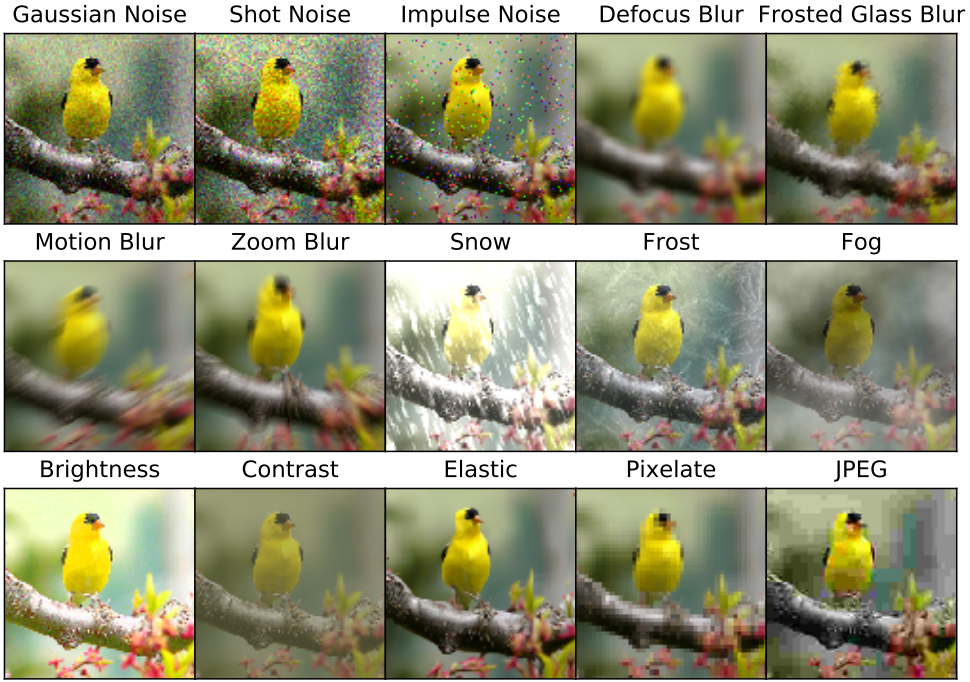
\includegraphics[width=0.9\textwidth]{gfx/fig1.png}  	  	 
	\caption[IMAGENET-C dataset consists of 15 types of corruptions]{Algorithmically generated corruptions categorized into digital, weather, blur, and noise distortions, each with varying severity levels~\cite{hendrycks2019benchmarking}.}
	\label{fig:imagenetC}
\end{figure}

Despite these advances in image-based benchmarking, equivalent structured robustness benchmarks for time-series data, particularly EEG signals, remain underdeveloped. EEG data's distinct temporal and spectral structures limit the applicability of image-based benchmarks, complicating the evaluation of model robustness in clinical EEG diagnostics like seizure detection, where noise, electrode dropouts, and artifacts pose significant challenges to diagnostic accuracy and reliability \cite{iwana2021empirical, lawhern2018eegnet}.

Thus, the establishment of dedicated EEG robustness benchmarks is essential for ensuring reliable and safe deployment of clinical EEG-based diagnostic systems.

\subsection{Methods to Improve Robustness and Calibration}
To address these robustness challenges, various general approaches have emerged within the machine learning community, aimed at enhancing model generalization and calibration under distributional shifts.

Regularization techniques are foundational, reducing overfitting by limiting model complexity and training convergence. Approaches such as weight decay, dropout, and early stopping effectively prevent neural networks from overfitting training data \cite{srivastava2014dropout, krogh1992simple}. Adversarial training, another critical regularization approach, introduces adversarially perturbed samples during training, significantly improving model resistance to adversarial inputs and data corruptions \cite{madry2017towards}.

Ensemble methods aggregate multiple model predictions, reducing variance and enhancing robustness. Approaches like bagging, boosting, and stacking combine diverse predictions, leading to improved calibration and stability by averaging individual model biases and errors \cite{lakshminarayanan2017simple}.

Bayesian neural networks quantify predictive uncertainty explicitly, utilizing probabilistic methods such as Monte Carlo dropout and variational inference. These methods provide calibrated predictions and reliable uncertainty estimates, essential for informed decision-making in critical applications \cite{gal2016dropout, blundell2015weight}.

Self-supervised learning methods further enhance robustness by learning generalizable feature representations without explicit supervision. Techniques such as contrastive learning and autoencoder-based methods effectively improve robustness to distributional shifts, particularly valuable when labeled data is scarce or noisy \cite{chen2020simple, grill2020bootstrap}.

Additionally, post-hoc calibration approaches like temperature scaling, isotonic regression, and Platt scaling adjust predicted probabilities, significantly enhancing confidence estimate reliability in high-stakes scenarios \cite{guo2017calibration}.

Despite broad coverage in general machine learning literature, these techniques remain insufficiently explored specifically for clinical EEG-based time-series analysis, marking a clear research gap that requires further exploration.

\subsection{Data Augmentation in Time Series}
Data augmentation has been instrumental in improving robustness and generalization in computer vision through techniques like flipping, rotation, scaling, cropping, and color jittering \cite{shorten2019survey}. However, directly applying such augmentations to time-series data is challenging due to inherent temporal dependencies and physiological constraints.

Time-series-specific augmentations have been proposed, including temporal jittering, scaling, permutation, and window slicing, preserving meaningful temporal structures \cite{iwana2021empirical}. Additionally, frequency-domain augmentations, notably SpecAugment, mask contiguous frequency and time segments, effectively enhancing robustness to noise and distortions \cite{spectral_aug}.

Advanced augmentation methods involve synthetic data generation using generative adversarial networks (GANs), generating plausible synthetic time-series data to mitigate class imbalance \cite{esteban2017realvalued}. Moreover, adapted mixup techniques generate virtual samples through interpolation, promoting smoother decision boundaries and improved generalization in time-series applications \cite{um2017data}.

In EEG classification, however, data augmentation is applied inconsistently, limiting reproducibility and systematic evaluation. While techniques like random cropping and channel shuffling have shown potential, standardized and comprehensive evaluations under corrupted conditions remain scarce.

Consequently, developing standardized evaluation frameworks for EEG-specific augmentation methods is crucial, ensuring robust, reproducible, and clinically relevant EEG classification systems.


%***********Contributions**********
\section{This Work's Contributions}
This work presents several key contributions toward improving the robustness and calibration of deep neural networks for EEG time series classification:

\begin{itemize}
    \item \textbf{EEG Corruption Benchmark:} To address the lack of standardized evaluation protocols for robustness in EEG classification, this work introduces a novel benchmark comprising controlled corruptions such as Gaussian noise, spectral augmentation, channel dropout, and signal dropout, explicitly designed to simulate real-world EEG imperfections encountered in clinical settings.

    \item \textbf{Systematic Robustness Evaluation:} Using the proposed benchmark, this work conducts a comprehensive assessment of state-of-the-art robustness enhancement techniques, including Mixup, Manifold Mixup, Multi-Input Multi-Output (MIMO), and Test-Time Adaptation (TTA).

    \item \textbf{Calibration Analysis and Metrics:} This work rigorously evaluates both predictive performance and confidence reliability using metrics such as accuracy, F1 score, and Expected Calibration Error (ECE), providing a nuanced understanding of model behavior under distributional shifts.

    \item \textbf{Method Compatibility and Combination Effects:} In addition to isolated evaluations, this work explores how robustness techniques interact when combined. Notably, performance degradation in specific combinations (e.g., MIMO with Manifold Mixup) highlights the importance of compatibility-aware design.
\end{itemize}
\begin{figure}[h!]
	\centering
        \def\svgwidth{400pt}
        \fontsize{7pt}{7pt}
 	\import{gfx/}{approach.pdf_tex} 	  	 	
	\caption[Overview of the structure of this work]{Overview of the structure of this work.}
	\label{fig:approach}
\end{figure}

\subsection*{This Work’s Structure}
This work is organized as follows. Chapter~\ref{ch:background} introduces the foundational concepts relevant to this work, including EEG, neural networks, calibration, and robustness. Chapter~\ref{ch:methodology} presents the proposed methodology, detailing the dataset, preprocessing steps, robustness-enhancing model variants, and the corruption techniques used to simulate real-world EEG imperfections. Evaluation protocols and calibration metrics are also discussed. Chapter~\ref{ch:results} reports the experimental results, focusing on performance under distribution shifts, calibration behavior, and the effects of method combinations. Chapter~\ref{ch:discussion} provides a critical discussion of findings and limitations. Finally, Chapter~\ref{ch:closure} concludes this work and outlines potential directions for future research.


%*****************************************
\chapter{Fundamentals}
\label{ch:background}
%*****************************************
This chapter provides the foundational knowledge required to understand the technical contributions of this work. It begins by introducing the biological basis of neural computation, followed by a discussion of epilepsy and electroencephalography (EEG) in clinical diagnostics. Next, the chapter presents core concepts in machine learning, including gradient-based optimization and deep learning. The final sections introduce calibration and robustness, two critical properties that influence the reliability of neural networks, particularly in real-world time-series analysis such as EEG classification.

\section{Neurons}
Neurons are the fundamental units of the nervous system responsible for transmitting, processing, and integrating information across the brain and body. Nearly every aspect of human cognition, sensation, movement, and emotion is orchestrated by the brain’s intricate network of approximately 86 billion neurons~\cite{Lent2012}. Each neuron forms thousands of synaptic connections with other neurons, giving rise to a complex and highly interconnected network that supports both local processing and large-scale communication across brain regions~\cite{Kandel2013, Sporns2011}.

Structurally, a typical neuron comprises three principal components: the soma (cell body), dendrites, and the axon (see Figure~\ref{fig:neurons}). The soma contains the nucleus and acts as the integrative center of the neuron. Dendrites extend from the soma and serve as receptive sites for incoming synaptic signals. The axon, often much longer than dendrites, transmits electrical impulses (action potentials) away from the soma toward other neurons, muscles, or glands~\cite{Purves2018}. The highly polarized structure of neurons enables unidirectional and efficient signal propagation, which is essential for coordinated neural computation.

\begin{figure}[htb]
	\centering
    \def\svgwidth{350pt}
 	\import{gfx/}{neuron.pdf_tex} 	 	
	\caption[Structure of a neuron]{Structure of a neuron. (Image source: Mauro Lanari\footnotemark. Accessed on 11th of May 2025.)}
	\label{fig:neurons}
\end{figure}
\footnotetext{\url{https://de.wikipedia.org/wiki/Nervenzelle}}

Functionally, neurons can be categorized by the type of signals they transmit. Excitatory neurons, which predominantly use the neurotransmitter glutamate, increase the likelihood of action potentials in downstream neurons. In contrast, inhibitory neurons release neurotransmitters such as γ-aminobutyric acid to suppress neuronal activity, thereby maintaining the balance necessary for stable and coordinated brain function~\cite{Kandel2013, Markram2004}. In addition to these, neuromodulatory neurons release chemicals like dopamine, serotonin, and acetylcholine~\cite{Kandel2013}. 
%A typical chemical synapse is shown in Figure~\ref{fig:synapse}, where neurotransmitters released from the presynaptic terminal bind to receptors on the postsynaptic membrane, initiating downstream electrical responses.

%\begin{figure}[htb]
%	\centering
%    \def\svgwidth{150pt}
% 	\import{gfx/}{synapse.pdf_tex} 	 	
%	\caption[Synaptic transmission between neurons]{Diagram of excitation %transmission at a chemical synapse from neuron A (presynaptic) to neuron B %(postsynaptic), showing vesicle release, receptor binding, and neurotransmitter %recycling~\cite{wikiSynapse}.}
%	\label{fig:synapse}
%\end{figure}

Neuronal structure and organization vary considerably across brain regions, reflecting their specialized functions. For instance, the cerebral cortex is organized into six laminar layers, each containing distinct neuron types and projection patterns critical for higher-order processing such as perception, decision-making, and language~\cite{Mountcastle1997}. In the hippocampus, neurons such as CA1 pyramidal cells and dentate gyrus granule cells play central roles in memory encoding and spatial navigation~\cite{Andersen2006}. The cerebellum, essential for motor coordination and adaptive learning, contains uniquely structured Purkinje cells characterized by elaborate dendritic trees enabling extensive synaptic input integration~\cite{Palay1974}.

One of the most critical features of neurons is their capacity for synaptic plasticity, the activity-dependent strengthening or weakening of synaptic connections. Synaptic plasticity underlies key cognitive functions such as learning and memory and is mediated by complex molecular mechanisms including long-term potentiation (LTP) and long-term depression (LTD)~\cite{Citri2008, Bliss1993}.

Despite their remarkable adaptability, neurons are particularly vulnerable to damage, degeneration, and dysfunction. Neurodegenerative disorders such as Alzheimer’s disease, Parkinson’s disease, and Huntington’s disease are characterized by progressive neuronal loss and synaptic failure, leading to severe impairments in cognition and motor function~\cite{DeKosky2004, Surmeier2017}. Moreover, psychiatric conditions including schizophrenia, major depressive disorder, and autism spectrum disorders are increasingly understood to involve disruptions in neuronal signaling, connectivity, or developmental trajectories~\cite{Insel2010, Courchesne2011}.

\section{Epilepsy}
Epilepsy is a chronic neurological disorder affecting approximately 50 million people globally, making it one of the most common brain disorders worldwide~\cite{whoEpilepsy}. It is characterized by a persistent predisposition to generate epileptic seizures and by the neurobiological, cognitive, psychological, and social consequences of this condition. A seizure is defined as a transient occurrence of signs and/or symptoms resulting from abnormal, excessive, or synchronous neuronal activity in the brain~\cite{fisher2014}.

Epileptic seizures can vary widely in manifestation depending on their origin and spread within the brain. Classification of seizures plays a crucial role in diagnosis and treatment planning. According to the International League Against Epilepsy (ILAE)~\cite{epilepsy2}: Seizures are classified into three major types based on the area of onset within the brain: focal onset, generalized onset, and unknown onset. 

Focal onset seizures originate within a specific, localized region of one cerebral hemisphere. These are manifest as focal aware seizures, where consciousness is preserved, or as focal impaired awareness seizures, where the patient experiences reduced awareness~\cite{epilepsy2}. Clinically, focal motor seizures can involve jerking, stiffening, or automatisms, while non-motor variants may involve sensory, emotional, or cognitive phenomena~\cite{fisher2017}.

In contrast, generalized onset seizures involve both cerebral hemispheres from the very beginning and result in immediate impairment of awareness~\cite{epilepsy2}. Sometimes, focal seizures evolve into generalized seizures, a phenomenon known as focal to bilateral tonic-clonic seizures. If the origin cannot be determined, e.g., due to a lack of clear symptoms or memory of onset, the seizure is classified as having an unknown onset~\cite{fisher2017}.

Figure~\ref{fig:seizure_flow} illustrates the standardized seizure classification used in clinical and research settings. This framework allows neurologists to better identify epilepsy syndromes and tailor treatments to specific seizure patterns.

\begin{figure}[htb]
	\centering
    \def\svgwidth{420pt}
    \fontsize{9pt}{9pt}
 	\import{gfx/}{ilae.pdf_tex} 	 	
	\caption[ILAE Seizure Classification Flowchart]{ILAE classification of seizure types (basic version) based on onset, awareness, and motor features~\cite{epilepsyDiagram}.}
	\label{fig:seizure_flow}
\end{figure}

\section{Electroencephalography (EEG)}
Electroencephalography (EEG) is a non-invasive neurophysiological method used to record the brain’s spontaneous electrical activity over time. This activity is generated by postsynaptic potentials of neurons, particularly from cortical pyramidal cells, and is measured using electrodes placed on the scalp~\cite{niedermeyer2005}.

EEG signals are recorded as voltage differences between electrode pairs placed on the scalp, typically measured relative to a reference. These differences reflect the summed postsynaptic potentials of large populations of cortical neurons, as individual neurons generate weak signals that are not detectable at the scalp level~\cite{niedermeyer2005}. To ensure consistent and anatomically informed electrode placement, the international 10–20 system is widely adopted for surface EEG. This system positions electrodes at intervals of 10\% or 20\% of the skull’s surface dimensions relative to anatomical landmarks~\cite{jurcak2007}, with each site labeled according to the underlying brain region (e.g., F for frontal, T for temporal). A schematic overview of this layout is shown in Figure~\ref{fig:electrodemap}.

\begin{figure}[h!]
	\centering
    \def\svgwidth{320pt}
    \fontsize{8pt}{8pt}
 	\import{gfx/}{channel10.pdf_tex} 	 	
	\caption[EEG 10-20 electrode map]{Exemplary layout of scalp electrodes based on the 10-20 system.}
	\label{fig:electrodemap}
\end{figure}

The electrical potential can be measured between a fixed reference and an active electrode (unipolar montage), or between two active electrodes (bipolar montage), depending on the acquisition setup. Due to the attenuating effects of the skull and scalp, surface EEG primarily reflects neural activity from superficial cortical regions and is less sensitive to deep brain structures. Despite these limitations, the spatial distribution of electrodes enables monitoring of regional dynamics across the cortex, which is critical for detecting pathological brain activity such as epileptic seizures.

An example of raw EEG signals from six bipolar channels over a 20-second interval is illustrated in Figure~\ref{fig:multi_channel}. These signals demonstrate the spatial variability of neural activity across different regions of the brain, as captured by the respective electrode pairs.

\begin{figure}[h!]
	\centering
    \def\svgwidth{420pt}
 	\import{gfx/}{eeg_plot.pdf_tex} 	 	
	\caption[Exemplary 20 seconds of six different EEG channels]{Exemplary 20-second interval of EEG recordings from six bipolar channels.}
	\label{fig:multi_channel}
\end{figure}

EEG rhythms are classified by their frequency bands: delta (0.5–4 Hz), theta (4–8 Hz), alpha (8-13 Hz), beta (13–30 Hz), and gamma (>30 Hz)~\cite{niedermeyer2005}. These rhythms correlate with different physiological and pathological brain states. For instance, delta waves dominate during deep sleep, while alpha waves appear when a person is awake but relaxed~\cite{niedermeyer2005}.

During a seizure, EEG signals often exhibit increased activity, which typically manifests as higher amplitude, altered frequency patterns, or sudden rhythmic discharges~\cite{seizuresurvey}. These patterns are critical for identifying seizure onset and distinguishing it from background activity.

Figure~\ref{fig:seizure_interval} presents a 50-second recording from the FP1–F7 channel where the seizure onset is clearly visible in the initial segment, marked by a sharp increase in signal amplitude and frequency content.

\begin{figure}[h!]
	\centering
    \def\svgwidth{400pt}
 	\import{gfx/}{seizure_interval.pdf_tex} 	 	
	\caption[EEG channel FP1–F7 around seizure onset]{Segment of EEG signal recorded from channel FP1–F7, showing a 50-second interval relative to seizure onset. The seizure activity (in red) is characterized by a rapid increase in amplitude and higher frequency fluctuations compared to the surrounding normal activity (in blue).}
	\label{fig:seizure_interval}
\end{figure}

\section{Machine Learning}
Machine learning (ML) is a subfield of artificial intelligence concerned with the development of algorithms and statistical models that enable systems to learn patterns from data and make predictions or decisions without being explicitly programmed~\cite{mitchell1997machine}. In a formal sense, machine learning can be viewed as the process of learning a function $f: \mathcal{X} \rightarrow \mathcal{Y}$ that maps input features $x \in \mathcal{X}$ to outputs $y \in \mathcal{Y}$, based on observed data $(x_i, y_i)_{i=1}^n$ drawn from a joint distribution $P(X, Y)$~\cite{bishop2006pattern}.

Machine learning models can be broadly categorized into three types based on their objective and data availability:

\begin{itemize}
\item Supervised learning: The model learns a mapping from inputs to known outputs using labeled data. The objective is to minimize a loss function $\mathcal{L}(f(x), y)$ that quantifies the discrepancy between predicted and actual outputs. Applications include classification and regression tasks~\cite{hastie2009elements}.

\item Unsupervised learning: The model receives only input data without labels and aims to uncover the underlying structure, such as clusters or latent representations, within the data. Common approaches include clustering, dimensionality reduction, and generative modeling~\cite{bishop2006pattern}.

\item Reinforcement learning: The model interacts with an environment and learns a policy $\pi(a|s)$ that maximizes cumulative reward over time by receiving feedback in the form of reward signals~\cite{sutton2018reinforcement}.
\end{itemize}

\begin{figure}[h!]
	\centering
    \def\svgwidth{350pt}
    \fontsize{8pt}{8pt}
 	\import{gfx/}{supervise.pdf_tex} 	 	
	\caption[Illustration of supervised learning]{Illustration of supervised learning. The model is trained on labeled data.}
	\label{fig:supervise}
\end{figure}
\begin{figure}[h!]
	\centering
    \def\svgwidth{350pt}
    \fontsize{8pt}{8pt}
 	\import{gfx/}{unsupervise.pdf_tex} 	 	
	\caption[Illustration of unsupervised learning]{Illustration of unsupervised learning. The model operates on unlabeled data.}
	\label{fig:unsupervise}
\end{figure}

Figures~\ref{fig:supervise} and~\ref{fig:unsupervise} provide intuitive visualizations of supervised and unsupervised learning paradigms, respectively. These examples highlight the fundamental difference in how information is used during training: while supervised models rely on labeled data to guide learning, unsupervised models must discover structure purely from the input space.

Another important distinction is between \textit{discriminative} and \textit{generative} models~\cite{Murphy}:

\begin{itemize}
\item Discriminative models learn the conditional probability $P(y|x)$ or a direct decision boundary between classes. They focus solely on prediction accuracy and include models such as logistic regression and support vector machines.

\item Generative models aim to model the joint distribution $P(x, y)$ and can generate new samples. They can be used both for prediction and for synthesizing data. Examples include Naive Bayes and Gaussian Mixture Models (GMMs)~\cite{bishop2006pattern}.
\end{itemize}
\subsection{Gradient Descent}
Gradient descent is a first-order iterative optimization algorithm widely used to minimize objective functions in machine learning, especially empirical loss functions over data distributions~\cite{gd}. Given a dataset $\mathcal{D} = \{(x_i, y_i)\}_{i=1}^N$, a predictive model $g_{\theta}(x)$ with learnable parameters $\theta \in \Theta$, and a loss function $\mathcal{L}(g_{\theta}(x), y)$, the goal is to minimize the empirical risk~\cite{bottou2012stochastic}:

\begin{equation}
R_{\mathcal{L}}(g_{\theta}) = \frac{1}{N} \sum_{i=1}^{N} \mathcal{L}(g_{\theta}(x_i), y_i)
\end{equation}

where $R_{\mathcal{L}}(g_{\theta})$ represents the average discrepancy between predictions and ground truth values.

The optimal parameters $\hat{\theta}$ are estimated by solving the minimization problem~\cite{ruder2016overview}:

\begin{equation}
\hat{\theta} = \arg \min_{\theta \in \Theta} R_{\mathcal{L}}(g_{\theta})
\end{equation}

Under standard regularity conditions (e.g., if $R_{\mathcal{L}}(g_{\theta})$ is twice continuously differentiable and the Hessian $\text{Hess}_{\theta}(R_{\mathcal{L}})$ is positive definite), $\hat{\theta}$ is guaranteed to be a local minimizer.

Gradient descent updates the parameters in the direction of the negative gradient of the loss function~\cite{lee2016gradient}:

\begin{equation}
\theta^{(k+1)} = \theta^{(k)} - \eta \nabla_{\theta} R_{\mathcal{L}}(g_{\theta})\big|_{\theta^{(k)}}
\end{equation}

where $\eta > 0$ is the learning rate, a hyperparameter controlling the step size. Choosing $\eta$ appropriately is critical: if it is too large, the updates may overshoot; if too small, convergence becomes slow.
\begin{figure}[h!]
	\centering
    \def\svgwidth{320pt}
 	\import{gfx/}{gradient.pdf_tex} 	 	
	\caption[Gradient Descent Trajectory]{Visualization of gradient descent optimization on a convex quadratic cost function. The arrows represent the iterative updates of the parameters $(\theta_0, \theta_1)$, moving in the direction of steepest descent.}
    \label{fig:gd_quadratic}
\end{figure}

In convex optimization problems, gradient descent converges to a global minimum, provided a proper learning rate is used~\cite{bottou2010large}. However, many modern machine learning models involve non-convex loss surfaces (e.g., in neural networks), where multiple local minima, saddle points, and flat regions exist~\cite{bottou2012stochastic}. In such cases, convergence to the global optimum cannot be guaranteed, but practical success is often achieved through careful tuning, initialization, and the use of stochastic variants~\cite{bottou2012stochastic}.

To address the computational challenges of large datasets, mini-batch gradient descent is often employed. Instead of computing gradients over the entire dataset, it uses small, randomly sampled subsets (batches), reducing memory consumption and introducing noise that can help escape shallow local minima~\cite{gd}.

\begin{equation}
\theta^{(k+1)} = \theta^{(k)} - \eta \nabla_{\theta} R^{(B)}_{\mathcal{L}}(g_{\theta})
\end{equation}

where $R^{(B)}_{\mathcal{L}}$ denotes the empirical risk computed on a mini-batch $B \subset \mathcal{D}$.
\subsection{Deep Learning}
Deep learning is a subfield of machine learning that studies models composed of multiple layers of nonlinear processing units, typically known as artificial neural networks (ANNs)~\cite{lecun2015deep}. When these networks contain two or more hidden layers, they are referred to as deep neural networks (DNNs)~\cite{lecun2015deep}.

An artificial neural network (ANN) is a computational graph consisting of interconnected units called neurons, organized into layers~\cite{lecun2015deep}. A typical feedforward neural network comprises an input layer, one or more hidden layers, and an output layer, as illustrated in Figure~\ref{fig:NN}.
\begin{figure}[h!]
	\centering
        \def\svgwidth{330pt}
 	\import{gfx/}{neuralNetwork.pdf_tex} 	  	 	
	\caption[A simple feedforward neural network with one hidden layer]{A simple feedforward neural network with one hidden layer.}
	\label{fig:NN}
\end{figure}
Each neuron performs a weighted summation of its inputs and applies a nonlinear activation function~\cite{goodfellow2016deep}:
\begin{equation}
a^{(l)} = \phi \left(W^{(l)} a^{(l-1)} + b^{(l)} \right)
\end{equation}

Here, $a^{(l)} \in \mathbb{R}^{n_l}$ represents the activations in the $l$-th layer, $W^{(l)} \in \mathbb{R}^{n_l \times n_{l-1}}$ is the weight matrix, $b^{(l)}$ is the bias vector, and $\phi$ is a non-linear function such as ReLU, sigmoid, or tanh. The network transforms an input $x \in \mathbb{R}^d$ through successive layers until a final prediction is produced.

\subsubsection{Training Neural Networks}
Training involves adjusting the weights $W^{(l)}$ and biases $b^{(l)}$ to minimize a predefined \textit{loss function}, typically via gradient-based optimization. The most common algorithm is Stochastic Gradient Descent (SGD) or its variants (e.g., Adam, RMSProp), which update parameters using the gradient of the loss with respect to each weight~\cite{bottou2012stochastic}:

\begin{equation}
W^{(l)} \leftarrow W^{(l+1)} - \eta \frac{\partial \mathcal{L}}{\partial W^{(l)}}
\end{equation}

Where $\eta$ is the learning rate and $\mathcal{L}$ the loss (e.g., cross-entropy for classification tasks). The gradient is computed efficiently via backpropagation, a recursive application of the chain rule from the output layer to the input layer~\cite{rumelhart1986learning}.

\subsubsection{Types of Neural Network Architectures}
The architecture of a neural network defines how data flows through layers of interconnected units to produce a prediction. Different architectural paradigms have been proposed to address specific data structures and learning tasks, each offering unique inductive biases and computational advantages.
\subsubsection{1. Fully Connected Networks (FCNs)}
Fully connected networks, also known as multilayer perceptrons (MLPs), are the most basic form of feedforward neural networks. In an FCN, each neuron in a layer is connected to every neuron in the preceding layer. Given an input vector $x \in \mathbb{R}^d$, the output of the first hidden layer is computed as~\cite{dl}:

\begin{equation}
a^{(1)} = \phi(W^{(1)}x + b^{(1)})
\end{equation}

Where $W^{(1)} \in \mathbb{R}^{n \times d}$ is the weight matrix, $b^{(1)}$ is a bias, and $\phi(\cdot)$ is a non-linear activation function. This process is repeated across layers to map the input to the final output.

Although FCNs are universal approximators~\cite{hornik1989multilayer}, they suffer from scalability issues when input dimensions are high, as the number of parameters grows quadratically with layer width. Moreover, they do not exploit local structures in data (e.g., temporal locality in EEG), making them suboptimal for time-series and spatially correlated inputs.

\subsubsection{2. Convolutional Neural Networks (CNNs)}
CNNs are specialized neural networks designed to capture \textit{local correlations} by applying learnable convolutional kernels across structured input spaces. For a two-dimensional input \( a^{(l-1)} \in \mathbb{R}^{H \times W} \) (e.g., an EEG spectrogram), the output of a convolutional layer at position \( (i, j) \) is computed as~\cite{dl}:

\begin{equation}
a_{i,j}^{(l)} = \phi \left( \sum_{m=0}^{M-1} \sum_{n=0}^{N-1} w_{m,n}^{(l)} \cdot a_{i+m,j+n}^{(l-1)} + b^{(l)} \right)
\label{eq:conv2d}
\end{equation}

Here, \( w_{m,n}^{(l)} \) denotes the kernel weight at position \( (m,n) \), \( \phi(\cdot) \) is a non-linear activation function (e.g., ReLU), and \( b^{(l)} \) is a bias term. The indices \( M \) and \( N \) represent the height and width of the kernel. This formulation assumes unit stride and zero padding unless otherwise specified.

In EEG signal processing, CNNs have been successfully applied to raw time-series data and to time-frequency representations like spectrograms~\cite{lawhern2018eegnet}. The local connectivity of CNNs enables them to learn frequency-band-specific and temporally localized patterns crucial for tasks such as seizure detection or mental state classification~\cite{lawhern2018eegnet}.
\begin{figure}[h!]
	\centering
        \def\svgwidth{400pt}
 	\import{gfx/}{cnn.pdf_tex} 	  	 	
	\caption[Visual representation of a 2D convolution operation]{Visual representation of a 2D convolution operation. A $2 \times 2$ kernel slides over a zero-padded $5 \times 5$ input matrix to produce a $4 \times 4$ output feature map. The highlighted region shows the first receptive field used to compute the top-left output value.}
	\label{fig:CNN}
\end{figure}
\subsubsection{3. Recurrent Neural Networks (RNNs)}
RNNs are designed for sequential data, where temporal dependencies are crucial. At each time step $t$, the hidden state $h_t$ is updated using the input $x_t$ and the previous hidden state $h_{t-1}$~\cite{roy2019chrononet}:

\begin{align}
h_t &= \phi(W_{xh}x_t + W_{hh}h_{t-1} + b_h) \\
y_t &= \psi(W_{hy}h_t + b_y)
\end{align}

Here, $W_{xh}, W_{hh},$ and $W_{hy}$ are learnable weight matrices, and $\phi$, $\psi$ are activation functions (e.g., tanh, softmax). Unlike FCNs or CNNs, RNNs retain a hidden memory across time, making them suited for tasks involving temporal context.

However, standard RNNs suffer from anishing and exploding gradient problems, limiting their ability to capture long-range dependencies. To address this, gated variants such as LSTMs and GRUs were introduced~\cite{hochreiter1997long, cho2014learning}, which use gating mechanisms to control information flow through time. In EEG classification, RNNs have been explored for capturing long-term brain signal dependencies, but their sequential nature limits parallelism and efficiency.

\subsubsection{4. Transformer-Based Architectures}
Transformer models were originally introduced for sequence modeling tasks in natural language processing~\cite{vaswani2017attention}, but their architecture has since been generalized to a variety of time-dependent domains, including multivariate time-series and biomedical signals. A key innovation of transformers is the use of \textit{self-attention mechanisms} to efficiently model global dependencies, overcoming the limitations of recurrent and convolutional architectures in capturing long-range interactions.

Let $x \in \mathbb{R}^{N \times D}$ denote the input sequence, where $N$ is the sequence length (e.g., number of EEG time steps) and $D$ is the feature dimension (e.g., number of channels or embeddings). A naive approach would be to flatten $x$ into a vector of size $N \cdot D$ and apply a fully connected layer. However, this leads to a parameter cost of $\mathcal{O}(N \cdot D \cdot M)$ for an output size $M$, which is prohibitively expensive for long sequences. Alternatively, using 1D convolutions requires only $\mathcal{O}(N \cdot M)$ parameters but lacks the capacity to model arbitrary long-range dependencies.

To address these challenges, the transformer architecture introduces \textit{multi-head self-attention}, which decomposes the input into \textit{queries} ($Q$), \textit{keys} ($K$), and \textit{values} ($V$) using learned linear projections~\cite{vaswani2017attention}. These are computed as:

\[
Q = xW^Q, \quad K = xW^K, \quad V = xW^V
\]

where $W^Q, W^K, W^V \in \mathbb{R}^{D \times d}$ are learnable projection matrices, and $d$ is the attention dimension. The core operation, known as \textit{scaled dot-product attention}, is defined as~\cite{vaswani2017attention}:

\begin{equation}
\text{Attention}(Q, K, V) = \text{softmax} \left( \frac{QK^\top}{\sqrt{d}} \right) V
\label{eq:attention}
\end{equation}

The matrix $QK^\top \in \mathbb{R}^{N \times N}$ computes pairwise similarity between input positions, and the softmax function normalizes these scores into a probability distribution. This allows each token in the sequence to attend to every other token, with learned relevance weights.

According to Vaswani et al.~\cite{vaswani2017attention}, in multi-head attention (shown in Figure~\ref{fig:multihead}), this mechanism is replicated $h$ times with different learned projections, allowing the model to jointly attend to information from different representation subspaces. The outputs of the $h$ heads are concatenated and projected through a final linear layer. Despite the quadratic complexity in sequence length ($\mathcal{O}(N^2)$), the overall parameter cost scales only with $\mathcal{O}(d^2)$, making it tractable even for long signals when combined with efficient attention variants.

\begin{figure}[h!]
	\centering
        \def\svgwidth{400pt}
 	\import{gfx/}{mutihead.pdf_tex} 	  	 	
	\caption[Visual representation of a 2D convolution operation]{Visual representation single attention head (left) and multi-head attention (right) consists of several attention layers~\cite{vaswani2017attention}.}
	\label{fig:multihead}
\end{figure}

\section{Calibration of Neural Networks}
In classification tasks, neural networks produce not only discrete labels but also confidence scores, typically derived from the softmax output layer. Ideally, these scores should reflect the true probability of correctness, a property known as \textit{calibration}.

Formally, a classifier is perfectly calibrated if~\cite{guo2017calibration}:
\begin{equation}
\mathbb{P}(Y = \hat{Y} \mid \hat{P} = p) = p, \quad \text{for all } p \in [0, 1]
\end{equation}
where $\hat{Y}$ is the predicted label, $\hat{P}$ the predicted confidence, and $Y$ the true label. For instance, if a model predicts 80\% confidence for a subset of samples, approximately 80\% of those should be correctly classified.

To quantify calibration, a widely adopted metric is the \textit{Expected Calibration Error (ECE)}, which partitions the confidence interval into $M$ bins and computes~\cite{ece}:
\begin{equation}
\text{ECE} = \sum_{m=1}^{M} \frac{|B_m|}{n} \left| \text{acc}(B_m) - \text{conf}(B_m) \right|
\end{equation}
where $B_m$ is the set of predictions in bin $m$, $\text{acc}(B_m)$ the empirical accuracy, and $\text{conf}(B_m)$ the average confidence~\cite{naeini2015obtaining, guo2017calibration}. A rigorous definition and implementation of ECE is provided in Chapter~\ref{ch:methodology}.

Recent work has shown that modern neural networks, particularly those with high capacity and limited regularization, often produce overconfident predictions and are thus poorly calibrated~\cite{guo2017calibration}. This degradation in calibration is frequently amplified by optimization techniques such as batch normalization and weight decay.

\subsubsection{Causes of Miscalibration}
The misalignment between predicted confidence and true correctness likelihood arises from several systemic factors.

First, overparameterization and extended training cycles tend to yield sharper softmax outputs, resulting in excessive confidence even on incorrect predictions~\cite{guo2017calibration}. Standard training objectives such as cross-entropy focus solely on minimizing prediction loss, without directly addressing confidence calibration.

Second, architectural choices, particularly batch normalization and ReLU activations, while effective for convergence, have been observed to amplify miscalibration, especially under distributional shift~\cite{ovadia2019can}.

Third, data-related factors such as class imbalance or label noise introduce skewed confidence scores, disproportionately affecting underrepresented or ambiguous instances~\cite{thulasidasan2019mixup}.

Finally, the absence of uncertainty-aware methods, such as Bayesian inference, deep ensembles, or stochastic regularization, restricts the model's ability to represent epistemic uncertainty, further impairing calibration~\cite{lakshminarayanan2017simple}.

\subsubsection{Post-Hoc Calibration}
A simple and effective post-processing method is \textit{temperature scaling}, which rescales logits using a learned scalar parameter $T > 0$~\cite{calibration1}:
\begin{equation}
P(\hat{y}) = \frac{\exp(z / T)}{\sum_j \exp(z_j / T)}  
\end{equation}
The temperature parameter $T$ is optimized on a validation set to minimize the negative log-likelihood (NLL). Larger values of $T$ soften the softmax distribution, reducing confidence without altering the predicted class~\cite{guo2017calibration}.

Due to its simplicity and empirical effectiveness, temperature scaling is widely used. However, it only modifies the model’s output at test time and does not address the underlying factors causing miscalibration during training.

\section{Robustness}
Robustness describes a model's ability to sustain predictive performance when exposed to inputs that differ from the training distribution. This capability is crucial in real-world applications, where variations such as noise, domain shifts, or hardware inconsistencies are common. 

A prominent benchmark for assessing corruption robustness is \textit{ImageNet-C}~\cite{hendrycks2019benchmarking}, which introduces 15 algorithmically generated perturbations applied to the ImageNet validation set. These include additive noise (e.g., Gaussian, impulse), blur (e.g., defocus, motion), weather artifacts (e.g., fog, snow), and digital distortions (e.g., JPEG compression). Each corruption is evaluated at five severity levels, enabling fine-grained analysis of model resilience.

Despite high clean accuracy, many state-of-the-art models experience significant performance degradation even under mild corruptions~\cite{hendrycks2019benchmarking}. This highlights a critical limitation of conventional generalization metrics. Furthermore, some models optimized for clean accuracy exhibit disproportionately poor robustness, revealing a robustness–accuracy trade-off not captured by standard evaluation.

An additional concern is the reliability of confidence estimates under shift. As shown by Ovadia et al.~\cite{ovadia2019can}, expected calibration error (ECE) often increases more rapidly than the decline in accuracy. Figure~\ref{fig:robust_calibration} illustrates this phenomenon: as corruption severity rises, model accuracy drops while ECE rises, indicating degradation in both performance and calibration.

\begin{figure}[h!]
	\centering
        \def\svgwidth{300pt}
 	\import{gfx/}{robust_calibration.pdf_tex} 	  	 	
	\caption[Robust Calibration Across Corruption Severity]{Robust Calibration Across Corruption Severity. As the corruption severity increases, model accuracy drops (blue) and expected calibration error (ECE) rises (red), indicating a decline in both predictive performance and confidence reliability.}
	\label{fig:robust_calibration}
\end{figure}

This dual degradation has motivated the development of methods targeting \textit{robust calibration}, wherein models are designed to maintain both high accuracy and reliable uncertainty estimates under distribution shift~\cite{ashukha2020pitfalls}.

%*****************************************
\chapter{Methods}
\label{ch:methodology}
%*****************************************
This chapter describes the experimental setup, including dataset preparation, corruption generation, and model training strategies. It details the methods used to benchmark robustness and calibration of EEG classification models under both clean and corrupted conditions. The chapter also outlines the evaluation metrics and training configurations used to compare the effectiveness of various robustness-enhancing techniques.

\section{Dataset and Preprocessing}
This work utilizes the Temple University Hospital Seizure Corpus (TUSZ), the largest publicly available EEG dataset for seizure detection research. TUSZ is widely adopted in the clinical and machine learning communities due to its scale, clinical authenticity, and comprehensive seizure annotations. The dataset consists of 19-channel scalp EEG recordings from 315 subjects, encompassing 1,791 annotated seizure events and over 797 hours of EEG recordings~\cite{seizureTUSZ}. Notably, TUSZ is the only publicly available corpus that includes multiple types of epileptic seizure events, making it uniquely suited for developing generalizable and clinically relevant detection models~\cite{seizureTUSZ}. The dataset exhibits a pronounced class imbalance, a common characteristic in clinical seizure corpora. Specifically, in the test set, only 5.55\% of EEG segments correspond to seizure events, with the remaining 94.45\% representing normal brain activity. This imbalance poses a significant challenge for neural network classifiers, as high accuracy can be trivially achieved by favoring the majority class, thus obscuring true model effectiveness. Understanding this imbalance is essential for interpreting performance metrics like precision, recall, and calibration under real-world conditions. Figure~\ref{fig:class_distribution} visualizes the class distribution in the TUSZ test set, providing essential context for the evaluation results reported in later sections.

\begin{figure}[h]
	\centering
    \def\svgwidth{300pt}
 	\import{gfx/}{class_distribution.pdf_tex} 	 	
	\caption[Class distribution of test set]{Class distribution of TUSZ test set.}
	\label{fig:class_distribution}
\end{figure}

Accurate classification of EEG data depends critically on robust preprocessing to mitigate variability and noise inherent to real-world clinical recordings. This work implements a structured preprocessing pipeline to standardize the input representation while preserving the clinically meaningful characteristics of the EEG. The pipeline consists of the following steps: montage extraction, notch filtering, resampling, segmentation, and spectrogram computation. An overview of these preprocessing stages is illustrated in Figure~\ref{fig:pipeline}, using a representative EEG channel.
\begin{figure}[h!]
	\centering
    \def\svgwidth{430pt}
    \fontsize{7pt}{7pt}
 	\import{gfx/}{preprocessing_pipeline_final.pdf_tex} 	 	
	\caption[Preprocessing pipeline for EEG signals]{Visualization of the preprocessing pipeline for a single EEG channel. Top to bottom: the raw bipolar signal, the signal after 60 Hz notch filtering, the resampled signal at 200 Hz, and the resulting time-frequency spectrogram. This pipeline transforms raw EEG into spectrally and temporally standardized input for downstream modeling.}
	\label{fig:pipeline}
\end{figure}
\subsubsection{Montage extraction}
EEG signals in the TUSZ corpus are recorded using heterogeneous reference schemes and channel configurations, leading to significant inter-subject and inter-session variability. To standardize input representations and reduce artifacts introduced by reference electrodes, this work converts all EEG recordings to a consistent bipolar montage. In this configuration, each signal is computed as the voltage difference between two predefined electrode pairs, which enhances the detection of localized brain activity and minimizes bias from reference placement~\cite{seizureTUSZ}. This preprocessing step ensures compatibility across recordings and preserves neurophysiologically meaningful signal characteristics for downstream analysis.

The electrode configuration is based on the International 10–20 system, which is widely used in clinical neurophysiology. After evaluating common EEG montages and based on guidelines from~\cite{tuszChannelSelection}, a consistent set of 19 electrodes was selected. The bipolar derivation for each channel is computed as the voltage difference between two electrodes:
\begin{equation}
M_k[t] = X_i[t] - X_j[t]
\end{equation}
where $M_k[t]$ denotes the $k$-th bipolar channel at time $t$, derived from electrodes $i$ and $j$, and $X_i[t]$, $X_j[t]$ are the corresponding time-domain signals. This differencing strategy captures localized voltage gradients while minimizing reference bias, facilitating robust seizure localization and inter-subject generalization~\cite{tuszChannelSelection}.

\subsubsection{Notch filtering}
EEG signals are frequently contaminated by narrowband interference from electrical power lines, typically at 50~Hz or 60~Hz, depending on the regional power grid. This interference can distort spectral characteristics and mislead frequency-domain analyses, making its removal an essential preprocessing step in EEG pipelines~\cite{notch}.

To suppress this periodic interference without significantly affecting adjacent frequency components, this work applies a second-order Infinite Impulse Response (IIR) notch filter to each EEG channel. The filter is designed to attenuate signals centered around 60~Hz with a high quality factor $Q$, which governs the sharpness of the notch.

The transfer function $H(z)$ of a second-order IIR notch filter is given by~\cite{notch}:
\begin{equation}
H(z) = \frac{1 - 2\cos(\omega_0)z^{-1} + z^{-2}}{1 - 2r\cos(\omega_0)z^{-1} + r^2 z^{-2}}
\end{equation}

Here,
\begin{itemize}
  \item $\omega_0 = \frac{2\pi f_0}{f_s}$ is the normalized notch frequency (e.g., $f_0 = 60$~Hz),
  \item $f_s$ is the sampling rate (250~Hz in this work),
  \item $r \in (0,1)$ is the pole radius controlling the filter’s bandwidth, which is related to the quality factor by 
  \[
  Q = \frac{f_0}{f_2 - f_1},
  \]
  \item and $f_1, f_2$ denote the -3~dB cutoff frequencies of the notch.
\end{itemize}

A high $Q$-factor (e.g., $Q = 30$) yields a narrow bandwidth, selectively attenuating 60~Hz interference while preserving physiological EEG components in nearby frequency bands.

\subsubsection{Resampling}
EEG recordings in the TUSZ dataset are sampled at different original rates, commonly 250 Hz, 512 Hz, or 1024 Hz, depending on acquisition hardware and protocol~\cite{zscore}. To ensure temporal consistency across subjects and facilitate uniform spectrogram computation, all EEG signals are resampled to 200 Hz.

Resampling is performed after filtering, using linear interpolation to compute intermediate values. This choice balances computational efficiency with sufficient temporal precision. The 200 Hz sampling rate preserves frequency content up to the Nyquist limit of 100 Hz, which is appropriate since most seizure-relevant EEG activity occurs below this threshold.

\subsubsection{Z-score Normalization}
After filtering and resampling, EEG signals are standardized using Z-score normalization. This step accounts for inter-patient variability and technical differences such as amplifier gain or electrode impedance, which can result in significant differences in signal amplitude across recordings~\cite{zscore}.

Normalization is performed per segment, where each segment is treated independently. For a given segment \text{X}, the normalized signal $X_{\text{norm}}$ is computed as~\cite{zscore}:
\begin{equation}
\centering
X_{\text{norm}} = \frac{X - \mu}{\sigma}
\label{eq:normalization}
\end{equation}
where $\mu$ and $\sigma$ are the mean and standard deviation of the EEG segment, respectively. This operation ensures that each input to the model has zero mean and unit variance, promoting numerical stability and faster convergence during training.

This work applies normalization to non-overlapping 5-second segments (corresponding to 1000 samples at 200 Hz), matching the temporal resolution used in the segmentation stage.

\subsubsection{Segmentation}
EEG signals are recorded as continuous time-series data, representing voltage variations captured over time. This time-domain representation directly reflects electrical brain activity as it evolves. However, neural network models typically require fixed-size inputs for efficient processing and consistent learning~\cite{eegsignal}. To meet this requirement, the continuous EEG recordings are segmented into short, uniform-length segments.

In this work, each segment is precisely 5 seconds long. Given the standardized sampling rate of 200 Hz, each segment comprises exactly 1000 data points (samples). When the total length of an EEG recording does not divide evenly into segments of this fixed length, the data is padded symmetrically at the start and end with zeros. This ensures every segment retains the same duration and the original temporal alignment of the EEG data is preserved.

Segmenting EEG recordings into uniform, short segments provides several benefits. It enables the neural network to learn efficiently by processing multiple EEG segments simultaneously during training (mini-batch processing)~\cite{EEGSignalAnalysis}. It also helps maintain a balanced representation of seizure and non-seizure segments within the dataset, supporting accurate modeling of seizure-related dynamics~\cite{EEGSignalAnalysis}. Lastly, segmenting the data emphasizes short-term temporal patterns essential for detecting the onset and progression of seizure activity~\cite{EEGSignalAnalysis}.

\subsubsection{Spectrogram Computation}
In seizure detection, examining how the frequency content of EEG signals changes over time is crucial, as abnormal patterns in specific frequency bands often mark seizures. Rather than analyzing EEG solely in the time or frequency domain, this work uses a time–frequency representation to preserve temporal and spectral information. A widely used technique is the spectrogram, which reflects how the signal’s power spectrum evolves over time~\cite{EEGSignalAnalysis}.

For each standardized EEG segment of 5 seconds (1000 samples at 200 Hz), a short-time Fourier transform (STFT) was computed separately for each EEG channel. Specifically, the spectrogram calculation used a 256-sample Hann window (corresponding to approximately 1.28 seconds) with a 50\% overlap (128 samples) between successive windows. This window length ensures that each overlapping interval is short enough to assume approximate stationarity of the EEG signal. Stationarity implies that the statistical properties of the EEG signals, such as mean and variance, remain relatively constant within each short segment. However, EEG signals are generally non-stationary due to rapidly changing neural dynamics~\cite{EEGSignalAnalysis}.

After computing the STFT, each segment produced a spectrogram, a 2D representation showing signal power across frequency (frequency bins) over time (timesteps). Each spectrogram was normalized to the range [0, 1] using min-max normalization. This normalization facilitates direct comparison of spectral energy distributions across segments and channels, regardless of amplitude variations.

The resulting channel-wise spectrogram for each EEG segment has dimensions determined by the STFT parameters: frequency bins × time steps. With a sampling rate of 200 Hz, a 256-sample window length (1.28 seconds), and a 128-sample overlap (0.64 seconds hop size), each 5-second EEG segment yields a spectrogram dimension of 129 frequency bins × 31 timesteps per channel.
\begin{figure}[htb]
	\centering
    \def\svgwidth{400pt}
 	\import{gfx/}{compare.pdf_tex} 	 	
	\caption[Comparison of Normal vs. Seizure Spectrograms]{Comparison of Normal vs. Seizure Spectrograms.}
	\label{fig:psd}
\end{figure}

This spectrogram-based transformation captures rich temporal and spectral cues essential for detecting epileptic activity. Numerous studies have shown that seizure events often exhibit characteristic bursts of high-frequency components (e.g., gamma band) and abrupt spectral shifts not present in baseline EEG~\cite{niedermeyer2005}. These pathological patterns are effectively captured by the time–frequency representation of the signal.

In contrast, non-seizure EEG typically displays more stationary spectral content, with energy concentrated in canonical frequency bands such as delta (0.5-4~Hz), theta (4–8~Hz), or alpha (8–13~Hz)~\cite{niedermeyer2005}. Figure~\ref{fig:psd} provides a visual example, highlighting the increased spectral variability during a seizure episode compared to a stable normal segment.
\clearpage
%---------------------------------------CORRUPTION-------------------------------------------
%---------------------------------------CORRUPTION-------------------------------------------
%---------------------------------------CORRUPTION-------------------------------------------
%---------------------------------------CORRUPTION-------------------------------------------
%---------------------------------------CORRUPTION-------------------------------------------
\section{Data Corruption Techniques}
To systematically evaluate the robustness of the models developed in this work, a suite of synthetic corruptions was applied to the held-out test set of the TUH EEG Seizure Corpus (TUSZ). These corruptions simulate real-world degradations commonly encountered in clinical and ambulatory EEG recordings, such as sensor failure, noise bursts, and frequency-specific signal distortions. Unlike traditional data augmentation, which enriches the training data to improve generalization~\cite{spectral_aug}, these techniques are applied exclusively to the test set, creating controlled distribution shifts to rigorously probe model behaviour under non-ideal conditions.

The corruptions are organized based on the domain in which they operate. Time-domain corruptions are applied directly to the raw EEG waveform, introducing temporal noise patterns or segment-level alterations. Frequency-domain corruptions manipulate the signal after a Fourier transformation, simulating spectral noise or band-specific interference. Lastly, time–frequency domain corruptions operate on the spectrogram representation, modifying both temporal and spectral features simultaneously.

Each corruption is parameterized by a severity level ranging from 1 (mild) to 5 (severe), following a standardized protocol inspired by the ImageNet-C framework~\cite{benchmarkingneuralnetworkrobustness}. In ImageNet-C, these severity levels were designed to evaluate model robustness under increasingly challenging perturbations. Adopting a similar approach, each corruption is applied to the EEG recordings at five predefined severity levels in this work, allowing for fine-grained robustness evaluation. The resulting test sets are collectively referred to as TUSZ-C (Corrupted TUSZ) and are used solely during inference to preserve a strict separation from training and validation data.

\subsection{Time-Domain Corruptions}
Time-domain corruptions operate directly on the raw EEG waveform~\cite{timedomain}. These perturbations simulate real-world signal artifacts caused by sensor detachment, hardware malfunction, patient movement, or environmental interference conditions commonly encountered in long-term or ambulatory EEG recordings. Unlike frequency-domain distortions, time-domain corruptions alter the morphology and continuity of the signal in its native representation, often degrading the temporal dynamics that models rely on to detect meaningful patterns such as seizure onsets or phase shifts~\cite{timedomain1}.

Prior works in robust speech recognition and physiological signal processing have shown that neural networks are particularly sensitive to waveform-level corruptions such as noise bursts, dropped segments, or amplitude distortions~\cite{timedomain1, timedomain2}. In this work, several synthetic time-domain corruptions are introduced to the test set to evaluate the resilience of the trained EEG models under temporal disruption. Each corruption is parameterized by severity and applied independently per sample, following a standardized protocol inspired by the ImageNet-C benchmark~\cite{benchmarkingneuralnetworkrobustness}.

\subsubsection{Signal Dropout}
Signal dropout is designed to mimic temporary loss of signal due to electrode detachment, motion artifacts, or transmission loss, phenomena commonly encountered in long-term EEG monitoring~\cite{timedomain1}. These dropouts may manifest as brief flatlines or zeroed-out intervals in the time series. For seizure detection or anomaly recognition systems, the ability to maintain reliable predictions under such conditions is crucial.

Let \( x \in \mathbb{R}^T \) denote a 1D EEG signal segment of duration \( T \) samples. Signal dropout is applied by randomly zeroing out multiple subsegments of the signal. The number, length, and location of these dropped intervals are sampled independently for each segment and corruption severity level.

The corrupted signal \( \tilde{x} \in \mathbb{R}^T \) is constructed as:

\begin{equation}
\tilde{x}_t = 
\begin{cases}
0, & \text{if } t \in \bigcup_{i=1}^{n} [s_i, s_i + l_i) \\
x_t, & \text{otherwise}
\end{cases}
\end{equation}

\noindent Where:
\begin{itemize}
  \item $n$: number of dropped intervals, computed so that the expected total dropped samples equals $\text{dropout\_prob}\times T$.  Concretely,
  \begin{equation}
      n \;=\;\left\lfloor\frac{\text{dropout\_prob}\times T}{\max(\text{min\_length},1)}\right\rfloor
  \end{equation}
  \item $s_i$: randomly chosen start time of the $i$-th dropout interval.
  \item $l_i$: uniformly sampled length of the $i$-th interval in $[\text{min\_length},\,\text{max\_length}]$.
  \item $x_t$: original signal at time $t$.
\end{itemize}

The corruption is controlled by three parameters: 
$\text{dropout\_prob} = 0.05 \times s$,  $\text{min\_length} = 0.1 \,\frac{s}{5}\,T$, and $\text{max\_length} = 0.2 \,\frac{s}{5}\,T$.

\noindent where \( s \in \{1, 2, 3, 4, 5\} \) is the severity level and \( T = 2500 \) samples (10s at 250 Hz). These parameters are used to control both the number and duration of dropped intervals, ensuring stronger degradation at higher severity.
\begin{figure}[h]
	\centering
    \def\svgwidth{420pt}
 	\import{gfx/}{signal_dropout_10s_segment.pdf_tex} 	 	
	\caption[Effect of signal dropout on a 10-second EEG segment]{Effect of Signal Dropout on a 10-second EEG segment. As severity increases, longer portions of the waveform are replaced with zeros, fully blanking the signal at severity 5.}
	\label{fig:signal_dropout}
\end{figure}

Figure~\ref{fig:signal_dropout} demonstrates the visual impact of signal dropout on a 10-second EEG segment. The topmost plot shows the raw, uncorrupted signal. The bottom left plot represents severity level 2, where a portion of the signal is dropped. The bottom rightmost plot, corresponding to severity level 5, shows a complete loss of signal content, simulating a worst-case sensor failure.

\subsubsection{Channel Dropout}
Channel dropout emulates the complete loss of signal from individual EEG electrodes, for example, owing to electrode detachment, motion artifacts, high contact impedance, or hardware failure, all of which occur frequently during long-term or ambulatory recordings \cite{channel_dropout1,channel_dropout4}.  
Unlike additive temporal noise, channel dropout operates in the \emph{spatial} domain: the entire waveform of a selected electrode is replaced by zeros, eliminating both temporal and spatial information from that channel~\cite{channel_dropout3}. Such corruption markedly deteriorates the performance of models that exploit inter-channel dependencies (e.g., spatial or graph convolutions) \cite{channel_dropout2,channel_dropout3}.

In this work, each channel is dropped independently according to a Bernoulli random variable whose success probability depends on the corruption \emph{severity level} \(s\in\{1,\dots,5\}\).  
Let \(\mathbf{x}\in\mathbb{R}^{C\times T}\) denote an EEG segment with \(C\) channels and \(T\) time samples. The corrupted segment \(\tilde{\mathbf{x}}\) is obtained as
\begin{equation}
\tilde{x}_{c}(t)=
\begin{cases}
0, & \text{with probability } p_{s},\\[4pt]
x_{c}(t), & \text{with probability } 1-p_{s},
\end{cases}\qquad
c=1,\dots,C,\;t=1,\dots,T,
\label{eq:channel_dropout}
\end{equation}
Where the dropout probability increases linearly with severity, \(p_{s}=0.1\,s\). Hence, at lower severities (\(s{=}1\),\(2\)) only a minority of electrodes are suppressed, preserving sufficient spatial structure for downstream analysis; higher severities induce widespread dropout and allow controlled stress-testing of spatial robustness.

\begin{figure}[h!]
    \centering
    \def\svgwidth{380pt}
    \import{gfx/}{channel_dropout.pdf_tex}
    \caption[Effect of Channel Dropout on a 10-s EEG segment]{Channel-dropout corruption applied to a 10-second EEG segment. The left column shows uncorrupted signals; the right column shows the corresponding corrupted signals at severity level \(2\).}
    \label{fig:channel_dropout}
\end{figure}

Figure~\ref{fig:channel_dropout} contrasts a 10-s raw EEG segment (left) with its corrupted counterpart at severity level \(s{=}2\) (right), where several but not all channels are completely silenced, mimicking the intermittent electrode reliability observed in practice.

\subsubsection{Gaussian Noise}
Gaussian noise is a classical corruption strategy in signal processing, commonly used to evaluate model robustness under additive stochastic perturbations. In the context of EEG, such noise mimics real-world sensor degradations including electromagnetic interference, unstable electrode contact, or analog-to-digital conversion artifacts~\cite{gaussian}.

Let \( \mathbf{x} \in \mathbb{R}^{C \times T} \) be an EEG segment with \( C \) channels and \( T \) time steps. We define the corrupted signal \( \tilde{\mathbf{x}} \) by additive zero-mean Gaussian noise:

\begin{equation}
\tilde{\mathbf{x}} = \mathbf{x} + \boldsymbol{\epsilon}, \quad \boldsymbol{\epsilon} \sim \mathcal{N}(0, \sigma_s^2)
\end{equation}

Here, \( \boldsymbol{\epsilon} \) represents independent and identically distributed (i.i.d.) noise applied to each element of the signal. The noise intensity \( \sigma_s \) is scaled by severity level \( s \in \{1,2,3,4,5\} \) according to:

\begin{equation}
\sigma_s = 0.1 \cdot s \cdot \mathrm{std}(\mathbf{x})
\end{equation}

This formulation ensures signal-relative perturbations that are linearly scaled in strength. Unlike fixed-standard-deviation noise, this approach adjusts to the signal's inherent amplitude, preserving comparability across EEG recordings with different baseline variances. Larger values of \( \sigma \) correspond to more intense noise corruption. The noise is applied independently across all channels and time steps, preserving the temporal structure while injecting high-frequency randomness.

\begin{figure}[htb]
	\centering
    \def\svgwidth{400pt}
 	\import{gfx/}{gaussian_noise.pdf_tex} 	 	
	\caption[Gaussian Noise corruption applied to a 10-second EEG segment]{EEG segment corrupted by Gaussian noise. Severity 2 introduces moderate perturbations, while severity 5 causes substantial distortion, reducing the visibility of fine-grained signal features.}
	\label{fig:gaussian}
\end{figure}

Following the ImageNet-C robustness protocol~\cite{benchmarkingneuralnetworkrobustness}, this method allows controlled corruption intensity from mild (severity 1) to highly disruptive (severity 5). Noise is applied independently across all channels and time steps, preserving the temporal structure while injecting high-frequency randomness that challenges feature extraction. Figure~\ref{fig:gaussian} illustrates the degradation of a 10-second EEG segment at severity levels 2 and 5.

\subsection{Frequency-Domain Corruptions}
While time-domain perturbations affect individual samples or local regions of the signal, frequency-domain corruptions operate globally on the signal's spectral representation. These techniques simulate artifacts such as hardware calibration errors, broadband interference, or physiological frequency drifts, which are common in real-world EEG acquisition setups. By manipulating the Fourier-transformed signal, one can systematically alter frequency content while preserving the temporal resolution of the original data~\cite{gaussian2}.
Let \( x[n] \in \mathbb{R}^T \) denote a single-channel EEG segment of length \( T \). Applying the real-valued inverse Discrete Fourier Transform (iDFT) yields a complex-valued frequency-domain representation~\cite{eeg}:

\begin{equation}
X[k] = \sum_{n=0}^{T-1} x[n] \cdot e^{-2\pi i \frac{kn}{T}}, \quad k = 0, \dots, \left\lfloor \frac{T}{2} \right\rfloor
\end{equation}

Each coefficient \( X[k] \in \mathbb{C} \) encodes the spectral content of the signal at frequency index \(k\), with its magnitude and phase representing the amplitude and phase shift of the corresponding sinusoidal component. Frequency-domain corruptions are applied by perturbing \( X[k] \) directly in the complex domain. The corrupted spectrum is then transformed back into the time domain using the inverse Discrete Fourier Transform (iDFT), preserving the temporal resolution while modifying global spectral characteristics.

\subsubsection{Gaussian Noise}
Gaussian noise injection in the frequency domain, implemented by transforming a time-series signal via the Fast Fourier Transform (FFT), perturbing its spectral components with noise, and inverting the transform, is theoretically equivalent to adding Gaussian noise directly in the time domain. This equivalence arises from the linearity property of the Fourier transform, where additive operations in the time domain correspond directly to additive operations in the frequency domain~\cite{gaussian2}. As a result, frequency-domain Gaussian noise does not introduce any fundamentally new corruption dynamics compared to its time-domain counterpart.

\subsection{Time-Frequency Domain Corruptions}
In signal processing, the \textit{time–frequency domain} refers to a representation where both time and frequency information are preserved simultaneously. Unlike the time domain, which reveals temporal changes, or the frequency domain, which describes spectral content aggregated over time, the time–frequency (TF) representation, such as a spectrogram, maps how the spectral properties of a signal evolve over time~\cite{timefreq}. This is particularly important in non-stationary signals like EEG, where neural oscillations and artifacts vary dynamically.

The most commonly used time–frequency transform for EEG is the Short-Time Fourier Transform (STFT), which partitions the signal into overlapping windows and computes the Fourier transform within each~\cite{timefreq}. This results in a 2D matrix \( S(f, t) \in \mathbb{R}^{F \times T} \), where \( f \) denotes frequency bins and \( t \) the temporal frames. This joint representation enables localised corruption, altering specific frequencies at specific times, mimicking realistic EEG degradation patterns such as intermittent sensor detachment or transient spectral distortions.

\subsubsection{Spectral Augmentation}
Spectral augmentation originates from the SpecAugment technique in speech processing~\cite{spectral_aug}. It introduces robustness by randomly masking or attenuating blocks of frequency and/or time in spectrograms. While initially proposed for mel-spectrograms in automatic speech recognition, this technique has been shown to generalize well to other domains, including EEG~\cite{spectral_aug}.

The method applies two primary forms of corruption:

\begin{itemize}
    \item Frequency masking: simulates dropout or attenuation in specific EEG bands (e.g., alpha: 8–12 Hz, beta: 12–30 Hz).
    \item Time masking: simulates temporal artifacts such as transient sensor failures or movement-induced dropouts.
\end{itemize}

This kind of corruption targets spectrotemporal robustness, allowing models to generalize better across varying frequency-localized noise profiles. In this work, spectral augmentation is applied as a synthetic corruption to test data, simulating real-world degradation localized in the spectrogram domain. The implementation proceeds as follows:
In this work, spectral augmentation is applied as a synthetic corruption to test data, simulating real-world degradation localized in the spectrogram domain. The implementation proceeds as follows:

\begin{enumerate}
    \item Spectrogram Computation: Each EEG segment \( x[n] \in \mathbb{R}^T \) is transformed into a magnitude spectrogram \( S(f, t) \in \mathbb{R}^{F \times T} \) using a Hann window of 256 samples (\( \approx 1 \) second at 250 Hz) with 50\% overlap. This yields approximately 129 frequency bins and 21 time frames per 10-second segment.

    \item Severity Parameterization: Inspired by the ImageNet-C corruption protocol~\cite{benchmarkingneuralnetworkrobustness}, five severity levels \( s \in \{1, 2, 3, 4, 5\} \) are defined. Each severity level determines:
    \begin{itemize}
        \item A frequency band \( [f_{\text{low}}, f_{\text{high}}] \) to be targeted (e.g., theta, alpha, beta).
        \item A reduction factor \( r = 1 - 0.1 \cdot s \), scaling down the energy in that band.
        \item A corruption probability \( p = 0.1 \cdot s \) controlling the likelihood of masking at each time frame.
    \end{itemize}

    \item Corruption Procedure: A binary mask is created over \( S(f, t) \), selecting both frequency rows and time columns probabilistically:
    \begin{equation}
    S_2(f, t) =
    \begin{cases}
        r \cdot S(f, t), & \text{if } f \in \text{band},\ t \sim \text{Bernoulli}(p) \\
        S(f, t), & \text{otherwise}
    \end{cases}
    \end{equation}

    This modifies only the selected time-frequency blocks, preserving the remaining signal integrity.

    \item Inverse Transformation (optional): Depending on the model, the corrupted spectrogram \( S_2(f, t) \) is either:
    \begin{itemize}
        \item Used directly as input (in spectrogram-based models), or
        \item Inverted via iSTFT to yield a corrupted time-domain signal \( \tilde{x}[n] \) (for waveform models).
    \end{itemize}
\end{enumerate}

\begin{figure}[h]
	\centering
    \def\svgwidth{220pt}
 	\import{gfx/}{specaug.pdf_tex} 	 	
	\caption[Spectral augmentation applied to a 10-second EEG segment]{Spectral augmentation applied to a 10-second EEG segment. Top: raw input; Bottom: severity level 2.}
	\label{fig:specaug}
\end{figure}

Figure~\ref{fig:specaug} illustrates the visual impact of spectral augmentation applied to a representative 10-second EEG segment. The leftmost panel shows the original, unaltered segment. The middle and right panels correspond to corrupted versions at severity level 2. Though the corruption occurs in the time–frequency domain, the resulting signal, after inverse STFT, is shown in the time domain, revealing subtle but structured waveform perturbations. These distortions reflect localized attenuation of EEG band power (e.g., in alpha or beta ranges) at random time frames, effectively simulating frequency-selective sensor errors.

\section{Model Variants}
\subsection{Multi-Input Multi-Output (MIMO)}

\subsubsection{Overview}
In traditional supervised learning, a neural network receives a single input (e.g., an EEG segment) and produces a corresponding single output (e.g., a binary seizure prediction). In contrast, the Multi-Input Multi-Output (MIMO) framework enables a neural network to process multiple inputs simultaneously and generate their respective predictions in parallel~\cite{mimofoundation}. This setup allows a single network to emulate an ensemble of subnetworks, thereby enhancing both predictive performance and robustness without requiring multiple separately trained models or additional inference overhead.

To illustrate the concept, consider a standard image classification task (shown in Figure~\ref{fig:mimo}), such as distinguishing between cats and dogs. In the conventional approach, each input image is processed individually to yield one prediction. However, in a MIMO setup, the network receives a batch of different images, e.g., a cat and a dog, and simultaneously produces predictions for both. Each input–output pathway functions as a virtual subnetwork. Although these subnetworks share the same core parameters, they are trained to solve the task independently, which fosters prediction diversity across heads.

At inference time, a single EEG segment is passed once through all MIMO heads in parallel. Each head, having been initialized and trained with different weight trajectories—constitutes a distinct subnetwork. Their M predictions are then averaged to yield the final output. No additional test‐time perturbations are required; diversity arises from the ensemble of subnetworks themselves~\cite{havasi2020training}. This mechanism approximates ensemble behavior within a single forward pass, making MIMO particularly attractive for time-sensitive applications such as clinical diagnostics, where computational efficiency and model reliability are both critical.

\begin{figure}[htb]
	\centering
    \def\svgwidth{350pt}
 	\import{gfx/}{mimo.pdf_tex} 	 	
	\caption[Illustration of the MIMO framework]{Illustration of the MIMO framework using an image classification example. Each input (e.g., cat or dog image) is passed through a shared network that simulates multiple independent subnetworks. During training, each input–output pair is treated as a distinct path (virtual head), allowing the model to produce separate predictions \( d_o, d_1 \)  for each input while sharing the same core parameters.}
	\label{fig:mimo}
\end{figure}

\subsubsection{Mathematical description}
To understand the core principles behind the MIMO strategy used in this work, we present a mathematical formulation inspired by Havasi et al.~\cite{modelMIMO}. While their formulation is model- and task-agnostic, it provides the theoretical foundation upon which the MIMO-based architecture in this work is adapted.

Let the training dataset consist of labeled EEG spectrogram segments:
\begin{equation}
\mathcal{D} = \left\{ \left(S^{(n)}, y^{(n)}\right) \right\}_{n=1}^{N}
\end{equation}
where each \( S^{(n)} \in \mathbb{R}^{C \times F \times T} \) denotes the spectrogram of the \( n \)-th EEG segment (with \( C \) channels, \( F \) frequency bins, and \( T \) time frames), and \( y^{(n)} \in \{0, 1\} \) is its binary seizure label.

In a conventional supervised learning setup, a neural network parameterized by \( \theta \) defines a probabilistic mapping:

\begin{equation}
p_{\theta}(\hat{y} \mid S)
\end{equation}

and is trained to minimize the expected negative log-likelihood loss (or another surrogate loss, such as focal loss) with a regularization term \( R(\theta) \):

\begin{equation}
\mathcal{L}(\theta) = \mathbb{E}_{(S, y) \sim \mathcal{D}} \left[ -\log p_{\theta}(y \mid S) \right] + R(\theta)
\end{equation}

In the Multi-Input Multi-Output (MIMO) configuration used in this work, the network is trained on \( M \) independently sampled spectrogram-label pairs per step:

\begin{equation}
\left\{(S_1, y_1), \ldots, (S_M, y_M)\right\} \sim \mathcal{D}
\end{equation}

At the input stage, these \( M \) spectrograms are concatenated along a new dimension, forming a tensor of shape \( M \times C \times F \times T \). Each input \( S_m \) is passed through a head-specific convolution layer, followed by a shared ResNet-18 backbone, and finally through a head-specific fully connected classifier. This yields \( M \) predictive distributions:

\begin{equation}
\left\{p_{\theta}(y_1 \mid S_1, \ldots, S_M), \ldots, p_{\theta}(y_M \mid S_1, \ldots, S_M)\right\}
\end{equation}

The total loss over a training step is the sum of the negative log-likelihood (or focal) losses for each subnetwork:

\begin{equation}
\mathcal{L}_M(\theta) = \mathbb{E}_{(S_1, y_1), \ldots, (S_M, y_M) \sim \mathcal{D}} \left[ \sum_{m=1}^{M} -\log p_{\theta}(y_m \mid S_1, \ldots, S_M) \right] + R(\theta)
\end{equation}

\begin{figure}[htb]
	\centering
    \def\svgwidth{400pt}
    \fontsize{8pt}{8pt}
 	\import{gfx/}{mimo_formulation.pdf_tex} 	 	
	\caption[Core concept of MIMO input-output mapping]{Illustration of the MIMO training setup.}
	\label{fig:mimo_formulation}
\end{figure}

A schematic overview of the MIMO configuration is shown in Figure~\ref{fig:mimo_formulation}. Independently sampled EEG spectrograms \( x_1, x_2, x_m \), each represented in the time-frequency domain, are jointly processed by a single MIMO neural network. The model outputs corresponding predictions \( y_1, y_2, y_m \).

This formulation allows each subnetwork (i.e., input-output pair within the shared model) to learn independently, encouraging diverse feature learning within a single training pass.

At inference time, a previously unseen EEG spectrogram \( S_0 \) is replicated \( M \) times to form:

\begin{equation}
S_1 = S_2 = \ldots = S_M = S_0
\end{equation}

The network outputs \( M \) independent predictions, each approximating the same conditional distribution. The final prediction is obtained by averaging the individual outputs:

\begin{equation}
p_{\theta}(y_0 \mid S_0) = \frac{1}{M} \sum_{m=1}^{M} p_{\theta}(y_m \mid S_0, \ldots, S_0)
\end{equation}

This enables robust, ensemble-like predictions in a single forward pass, substantially improving calibration and generalization, particularly for noisy or out-of-distribution EEG inputs.

\subsubsection{Learning Architecture}
The MIMO-based model employed in this work builds upon the general formulation described earlier. The goal is to leverage an ensemble's predictive diversity while maintaining computational efficiency through a single shared architecture.

The input to the model is a batch of EEG spectrogram segments, where each segment corresponds to a fixed-duration window of multichannel EEG signals. For each training iteration, $M$ independently augmented copies of the batch are created, representing $M$ diverse perspectives on the same data.

Each augmented input $X_m$ is first passed through a head-specific convolutional layer with a large 7×7 kernel. These initial layers allow each ensemble head to learn distinct low-level features. The resulting feature maps are then fed into a shared ResNet-18 backbone, which extracts high-level spatio-temporal representations through a series of residual blocks. The use of residual connections allows for stable training of deeper architectures by mitigating gradient vanishing~\cite{resnet}.
\begin{figure}[h!]
	\centering
    \def\svgwidth{130pt}
    \fontsize{8pt}{8pt}
 	\import{gfx/}{mimo_backbone.pdf_tex} 	 	
	\caption[MIMO Architecture Overview]{Overview of the MIMO ResNet-18 architecture.}
	\label{fig:mimo_architecture}
\end{figure}

After global average pooling, the shared features are distributed to head-specific fully connected (FC) layers, each of which produces a binary classification logit. This architectural design enables ensemble-like behavior by encouraging subnetworks to learn complementary decision boundaries while sharing most of the model parameters.

Figure~\ref{fig:mimo_architecture} illustrates this MIMO architecture, highlighting the modular flow from input spectrograms through shared and head-specific layers to ensemble outputs. During training, each head's prediction is supervised using the \textit{sigmoid focal loss}. Focal loss is particularly suitable for class imbalance, as it down-weights easy negatives and focuses training on harder examples:
\begin{equation}
\text{FL}(p_t) = -\alpha_t (1 - p_t)^{\gamma} \log(p_t)
\end{equation}
where \( \gamma \) is the focusing parameter and \( \alpha_t \) controls the weighting of classes.

The model is optimized using the Adam optimizer~\cite{adamOptimizer} with an initial learning rate of $1 \times 10^{-3}$, which is reduced adaptively based on validation performance. Training proceeds with a batch size of 32 and incorporates early stopping based on validation F1 score and loss trends. The training steps described above are formally summarized in Algorithm~\ref{alg:mimo_training}.

\begin{algorithm}[H]
\caption{Training Procedure for MIMO ResNet-18 Model}
\label{alg:mimo_training}
\begin{algorithmic}[1]
\Require Preprocessed EEG spectrogram dataset $\mathcal{D}$, number of ensemble heads $M$, initial learning rate $\eta$, epochs $E$, batch size $B$
\State Initialize model parameters $\theta$
\State Initialize optimizer (Adam) with learning rate $\eta$
\For{$\text{epoch} = 1$ to $E$}
  \For{each mini-batch $(X, Y) \in \mathcal{D}$}
    \Comment{Dataset-level corruption/augmentation}
    \State Apply chosen corruption/augmentation once to each sample in $X$
    
    \Comment{MIMO batch construction}
    \State Sample $M$ random permutations $\{\pi_1, \dots, \pi_M\}$ of $\{1, \dots, B\}$
    \For{$m = 1$ to $M$}
      \State $X^{(m)} \gets X[\pi_m]$ \hfill \Comment{Shape: $[B, C, F, T]$}
    \EndFor
    
    \Comment{Head-specific initial convolution}
    \For{$m = 1$ to $M$}
      \State $H_m \gets \text{HeadConv}_m(X^{(m)})$
    \EndFor

    \Comment{Shared backbone}
    \State $H_{\text{shared}} \gets \text{BackboneResNet18}\left( \sum_{m=1}^{M} H_m \right)$

    \Comment{Head-specific classifier}
    \For{$m = 1$ to $M$}
      \State $Z_m \gets \text{FC}_m(H_{\text{shared}})$ \hfill \Comment{Logits shape: $[B, 1]$}
    \EndFor

    \Comment{Loss and parameter update}
    \State $L_m \gets \text{FocalLoss}(Z_m, Y)$ for each $m$
    \State $L \gets \frac{1}{M} \sum_{m=1}^{M} L_m$
    \State Backpropagate $L$, update $\theta$
  \EndFor
  \State Validate on hold-out set, adjust $\eta$ or early-stop if needed
\EndFor
\State \Return Learned parameters $\theta$
\end{algorithmic}
\end{algorithm}

During training, each input is augmented with mild channel-wise Gaussian noise ($\sigma=0.01$). This augmentation is intended to promote diversity among the MIMO heads by introducing variation in the inputs according to Lakshminarayan et al.~\cite{lakshminarayanan2017simple}. However, since Gaussian noise is also used as a test-time corruption type, this introduces a form of data leakage that may inflate robustness results on that corruption. This is acknowledged in the discussion (Section~\ref{sec:limitations}).

\subsection{Manifold Mixup}
Manifold Mixup is a regularization technique that improves generalization and robustness in neural networks by interpolating hidden representations rather than raw inputs. While traditional Mixup~\cite{Mixup} generates virtual training examples by linearly combining input pairs and their corresponding labels in the input space, Manifold Mixup proposes to perform such interpolations at intermediate layers of the network~\cite{manifoldmixup}. This encourages the network to learn smoother decision boundaries in its learned feature space and has been shown to enhance performance on out-of-distribution and noisy inputs.

The core idea is to expose the model to interpolated feature representations during training, thereby regularizing the hidden manifolds of the model. By training on these augmented intermediate representations, the model avoids overfitting to high-confidence but brittle patterns and instead learns more semantically meaningful features.

\subsubsection{Mathematical description}
Let \((x_i, y_i), (x_j, y_j) \in \mathcal{D}\) be two randomly selected training examples from the dataset. A standard neural network defines a sequence of transformations \( f = f_k \circ f_{k-1} \circ \cdots \circ f_1 \), mapping the input \( x \) to output \( f(x) \). In Manifold Mixup, we select a layer \( l \in \{1, \ldots, k\} \) and apply interpolation to the features at that layer.

Let \( h_i = f_l(x_i) \) and \( h_j = f_l(x_j) \) be the intermediate representations at layer \( l \). We compute the mixed representation and label as:
\begin{equation}
\tilde{h} = \lambda h_i + (1 - \lambda) h_j, \quad \tilde{y} = \lambda y_i + (1 - \lambda) y_j
\end{equation}


where \( \lambda \sim \text{Beta}(\alpha, \alpha) \), with \( \alpha > 0 \) controlling the interpolation strength.

The remaining layers \( f_{l+1}, \ldots, f_k \) process \( \tilde{h} \) to yield predictions \( \hat{y} = f_k \circ \cdots \circ f_{l+1}(\tilde{h}) \), and the loss is computed against \( \tilde{y} \).

This encourages the model to produce meaningful outputs not only for training samples but also for interpolated representations in the hidden space, thereby improving generalization and robustness to out-of-distribution inputs.

\subsubsection{Architectural Integration and Learning Approach}
This section details how Manifold Mixup is integrated into the ResNet-18 architecture used in this work and how it is trained end-to-end on EEG spectrograms. Unlike standard input-level mixup, Manifold Mixup operates by interpolating hidden representations at randomly selected intermediate layers of the network. This yields a stronger regularization signal by enforcing linear behavior in deeper feature manifolds, which are closer to the decision boundaries.

Figure~\ref{fig:manifoldmixup} illustrates the architecture. At each training iteration, two samples \((x_i, y_i)\) and \((x_j, y_j)\) are drawn from the training batch. A layer \(k\) is selected at random from a predefined set of eligible mixup layers \(\mathcal{K}\), such as the output of residual block 1, 2, or 3. The model computes the forward pass up to layer \(k\) for both inputs, obtaining the intermediate hidden representations \(h_i^{(k)} = f_k(x_i)\) and \(h_j^{(k)} = f_k(x_j)\).

A mixing coefficient \(\lambda \sim \text{Beta}(\alpha, \alpha)\) is sampled, and the representations are linearly interpolated:

\begin{equation}
\tilde{h}^{(k)} = \lambda h_i^{(k)} + (1 - \lambda) h_j^{(k)}
\end{equation}

The mixed representation \(\tilde{h}^{(k)}\) is then propagated forward through the remaining network layers \(f_{>k}\) to obtain the logits \(\tilde{z} = f_{>k}(\tilde{h}^{(k)})\). The targets are similarly interpolated as:

\begin{equation}
\tilde{y} = \lambda y_i + (1 - \lambda) y_j
\end{equation}

For binary classification, labels are one-hot encoded vectors, and \(\tilde{y}\) remains a valid soft target. The model is trained to minimize the standard binary cross-entropy loss between \(\tilde{z}\) and \(\tilde{y}\).

To stabilize training, batch normalization statistics are frozen during mixup layers, and residual connections are preserved around the interpolated hidden states. Mixup is applied per-batch, not per-sample, and care is taken to ensure that EEG segments in a mixup pair originate from the same channel layout. This is critical in EEG settings, where inter-channel alignment carries physiological meaning.

Optimization is performed using the Adam optimizer with a base learning rate of \(1 \times 10^{-3}\), and early stopping based on validation F1-score. Mixup hyperparameter \(\alpha\) is set to 0.4 following the recommendation of Verma et al.~\cite{manifoldmixup}.
\begin{figure}[h!]
	\centering
    \def\svgwidth{300pt}
 	\import{gfx/}{manifold.pdf_tex} 	 	
	\caption[Overview of the Manifold Mixup learning process integrated into ResNet-18]{Overview of the Manifold Mixup learning process integrated into ResNet-18. Two EEG spectrograms \((x_i, y_i)\) and \((x_j, y_j)\) are independently passed through a shared ResNet-18 backbone.}
	\label{fig:manifoldmixup}
\end{figure}

 %A hidden representation \( h \) is extracted at a randomly selected intermediate layer (one of ResNet-18's four residual blocks). These representations are linearly interpolated along with their labels using a sampled mixing coefficient \( \lambda \sim \text{Beta}(\alpha, \alpha) \). The mixed representation is propagated through the remaining layers, and the model is trained to predict the mixed label.%

\subsection{MIMO + Manifold Mixup}

To combine the complementary strengths of two robustness strategies, multi-input multi-output (MIMO) ensembling and Manifold Mixup regularization, we adopt a joint MIMO–Manifold Mixup framework.  In contrast to treating mixup and ensembling separately, our model processes multiple distinct inputs in parallel through a shared backbone and applies Manifold Mixup within it.  This architecture builds on Havasi \emph{et al.}’s MIMO paradigm~\cite{modelMIMO} and Verma \emph{et al.}’s Manifold Mixup~\cite{manifoldmixup}, but their integration for EEG analysis has not previously been explored.

\subsubsection{Architecture Overview}
Given a mini-batch of \(B\) spectrograms \(\{x_i\}_{i=1}^B\), we first apply any dataset-level corruptions or augmentations \emph{once} per sample (e.g.\ channel noise, spectral masks).  To form an ensemble of \(M\) subnetworks, we generate \(M\) independent random permutations \(\{\pi_m\}_{m=1}^M\) of the batch indices and stack
\begin{equation}
X_{\mathrm{mimo}} = \bigl[x_{\pi_1(1)},\dots,x_{\pi_1(B)};\;\dots\;;\,x_{\pi_M(1)},\dots,x_{\pi_M(B)}\bigr]\;\in\;\mathbb{R}^{M\times B\times C\times F\times T}\,
\end{equation}

Each slice \(X_{\mathrm{mimo}}[m]\) is processed by a head-specific 7×7 convolution, then passed through the shared ResNet-18 backbone.

Within the backbone, at each training iteration we pick a random layer \(\ell\in\{0,1,2,3,4\}\) to perform Manifold Mixup.  Denote the intermediate features of two permuted heads at layer \(\ell\) by \(h_i\) and \(h_j\).  We interpolate
\begin{equation}
 \tilde{h} = \lambda\,h_i + (1-\lambda)\,h_j  
\end{equation}
\begin{equation}
\tilde{y} = \lambda\,y_i + (1-\lambda)\,y_j
\end{equation}
with \(\lambda\sim\mathrm{Beta}(\alpha,\alpha)\).  The mixed feature \(\tilde{h}\) then continues through the remaining backbone layers.

Finally, each of the \(M\) heads applies its own fully-connected layer to either the unmixed or the mixed feature (for heads \(i\) and \(j\), respectively), producing logits \(\hat y_1,\dots,\hat y_M\) (shown in Figure~\ref{fig:mimomanifoldmiup}).  At inference, we simply average those \(M\) predictions:
\[
\hat y = \frac1M\sum_{m=1}^M \hat y_m.
\]

\begin{figure}[h!]
	\centering
    \def\svgwidth{410pt}
    \fontsize{8pt}{8pt}
 	\import{gfx/}{mimomanifoldmixup.pdf_tex} 	 	
	\caption[Schematic of the combined MIMO + Manifold Mixup architecture.]{Schematic of the combined MIMO + Manifold Mixup architecture. Multiple augmented spectrogram inputs are processed through head-specific convolutions and a shared ResNet-18 backbone.}
	\label{fig:mimomanifoldmiup}
\end{figure}

\subsubsection{Training Procedure}
During each training step:

\begin{enumerate}
  \item Sample a batch \(\{(x_i,y_i)\}_{i=1}^B\) and apply any dataset-level corruptions once per \(x_i\).  
  \item Generate \(M\) random permutations \(\{\pi_m\}\) of \(\{1,\dots,B\}\) and stack into \(X_{\mathrm{mimo}}\in\mathbb{R}^{M\times B\times C\times F\times T}\).  
  \item Choose a random mixup layer \(\ell\in\{0,1,2,3,4\}\).  
  \item Forward \(X_{\mathrm{mimo}}\) through:
    \begin{itemize}
      \item Head-specific initial convolutions.  
      \item Shared ResNet-18 up to layer \(\ell\).  
      \item Manifold Mixup at \(\ell\): interpolate two head features and labels.  
      \item Remaining ResNet-18 layers.  
      \item Head-specific FC layers to produce \(\hat y_1,\dots,\hat y_M\).  
    \end{itemize}
  \item Compute two losses:
    \[
      \mathcal{L}_{\mathrm{head}}
      = \frac1M\sum_{m=1}^M\mathrm{FL}(\hat y_m,\,y),
      \quad
      \mathcal{L}_{\mathrm{mix}}
      = \mathrm{FL}(\hat y_{\mathrm{mix}},\,\tilde y).
    \]
  \item Total loss: \(\mathcal{L}_{\mathrm{total}} = \mathcal{L}_{\mathrm{head}} + \mathcal{L}_{\mathrm{mix}}.\)  
  \item Backpropagate \(\mathcal{L}_{\mathrm{total}}\) and update parameters via Adam.
\end{enumerate}

\noindent
This procedure ensures that each head learns from a distinct subset of the batch (MIMO diversity) and that Manifold Mixup smooths decision boundaries within the shared backbone.  No per-head augmentations are applied at inference; diversity arises solely from the learned subnetworks.

\section{Test-Time Adaptation}
Test-time adaptation (TTA) has recently emerged as a compelling paradigm for improving model performance under distribution shifts between training and testing conditions. As illustrated in Figure~\ref{fig:tta}, unlike conventional inference, where a pre-trained model’s parameters remain fixed, TTA allows a model to adjust its internal representations on unlabeled test data~\cite{TTA}.


In this work, we adopt the TENT algorithm.  TENT minimizes the prediction entropy  by~\cite{tta}:
\begin{equation}
\mathcal{L}_{\mathrm{entropy}}
= -\frac{1}{N}\sum_{i=1}^{N}\bigl[p_i\log p_i + (1-p_i)\log(1-p_i)\bigr]   
\end{equation}

Where \(p_i\) is the model’s predicted probability for the positive class on sample \(i\).  Crucially, following the original TENT implementation, we restrict adaptation to the affine scale and shift parameters of all BatchNorm layers, leaving the remaining weights frozen.  

\begin{figure}[h]
  \centering
  \def\svgwidth{0.8\columnwidth}
  \import{gfx/}{tta.pdf_tex}
  \caption[Overview of TENT-based test-time adaptation process]{Overview of TENT-based test-time adaptation process.}
  \label{fig:tta}
\end{figure}

\subsection*{Implementation Details}

We implement TENT in this work as follows:
\begin{itemize}
  \item Initialize an SGD optimizer over only the BatchNorm \(\{\gamma,\beta\}\) parameters.
  \item For each test batch/sample, perform \(K\) steps (typically \(K=1\)–3) of gradient descent on \(\mathcal{L}_{\mathrm{entropy}}\).  
  \item Recompute final predictions with the adapted model.
\end{itemize}

Restricting updates to BN parameters ensures (a) fast, label-free adaptation and (b) preservation of the core representations learned during training.  When evaluated on both clean EEG and the corrupted TUSZ‐C benchmark, TENT yields improved calibration and robustness under realistic noise and dropout artifacts.

While more recent TTA variants (e.g.\ SAR~\cite{ZHOU2024109974}, COME~\cite{tta2}) extend beyond entropy minimization or adapt deeper layers, we focus here on the original TENT algorithm as a lightweight, widely adopted baseline for EEG applications.

%-----------------------EVALUATION-------------------------
%-----------------------EVALUATION-------------------------
%-----------------------EVALUATION-------------------------
%-----------------------EVALUATION-------------------------
%-----------------------EVALUATION-------------------------
\section{Evaluation}
This chapter outlines the evaluation methodology adopted to assess the predictive performance and reliability of the neural models developed in this work. Given the emphasis on improving both robustness and calibration, the models were systematically tested across two key conditions: (i) the clean held-out test set from the preprocessed TUH EEG Seizure Corpus (TUSZ), and (ii) a synthetically corrupted version of this test set designed to simulate real-world distributional shifts, such as noise, channel dropout, or sensor artifacts encountered in clinical environments. Evaluation was performed using a combination of classification metrics (F1-score, accuracy) and probabilistic calibration metrics (expected calibration error), allowing for a multifaceted view of each model’s behavior under clean and perturbed conditions.

To compute the classification metrics, predictions are compared against ground truth labels using standard confusion matrix components: true positives (TP), false positives (FP), true negatives (TN), and false negatives (FN).

\subsection*{F1-Score}
The F1-score is a widely used metric for evaluating binary classifiers, particularly when class distributions are imbalanced~\cite{f1}. It combines two fundamental components of classification quality: precision and recall, into a single harmonic mean. This makes it especially useful in medical applications, such as EEG classification, where correctly identifying minority class instances (e.g., seizure or artifact) is critical.
Let the ground-truth labels be \( y_i \in \{0, 1\} \) and the model predictions be \( \hat{y}_i \in \{0, 1\} \), for all \( i = 1, \ldots, N \) samples in the test set.

We define the following terms:
\begin{itemize}
    \item True Positives (TP): Number of samples where \( y_i = 1 \) and \( \hat{y}_i = 1 \)
    \item False Positives (FP): Number of samples where \( y_i = 0 \) and \( \hat{y}_i = 1 \)
    \item False Negatives (FN): Number of samples where \( y_i = 1 \) and \( \hat{y}_i = 0 \)
\end{itemize}

From these counts, we compute: Precision, also known as the \textit{Positive Predictive Value}, measures the fraction of predicted positive instances that are actually correct~\cite{f1}:
\begin{equation}
\text{Precision} = \frac{\text{TP}}{\text{TP} + \text{FP}}
\end{equation}
A high precision indicates that when the model predicts the positive class, it is usually correct. Recall, also known as \textit{Sensitivity} or \textit{True Positive Rate}, quantifies the fraction of actual positive instances that are correctly identified~\cite{f1}:
\begin{equation}
\text{Recall} = \frac{\text{TP}}{\text{TP} + \text{FN}}
\end{equation}
A high recall implies that most of the true positive cases were recovered by the model. The F1-score balances precision and recall by computing their harmonic mean~\cite{f1}:
\begin{equation}
\text{F1} = \frac{\text{2.Precision.Recall}}{\text{Precision} + \text{Recall}}
\end{equation}
This score can take values between 0 and 1, with a high value indicating good model performance with high precision and high recall. This metric is particularly useful when the dataset is unbalanced and there is a risk that the model will be biased towards the more common class. In this work, the F1-score is used as a primary evaluation metric to assess model performance on both clean and corrupted EEG test data, offering a balanced view of how well the model detects true positive events while minimizing false alarms.

\subsection*{Accuracy}
In binary classification tasks such as those evaluated in this work, Accuracy is often the first metric used to assess a model's performance~\cite{accuracy}. It is defined as the proportion of correct predictions (both positive and negative) out of the total number of predictions~\cite{accuracy}:
\begin{equation}
\text{Accuracy} = \frac{\text{TP} + \text{FN}}{\text{TP} + \text{TN} + \text{FP} + \text{FN}}
\end{equation}
It provides an overall correctness score, which is useful in balanced datasets where all classes are equally represented. For example, in a task where the number of seizure and normal segments is roughly equal, a high accuracy implies good model performance across both classes.

However, in imbalanced datasets like those used in EEG classification tasks, where seizure events are rare, accuracy can give a misleadingly optimistic estimate. A trivial classifier that always predicts the majority class (e.g., “no seizure”) might still achieve high accuracy without correctly identifying any seizures.

\subsection*{Expected calibration error (ECE)}
While classification metrics such as accuracy and F1-score assess how often a model makes correct predictions, they do not capture how confident the model is in those predictions. In high-stakes domains such as clinical EEG analysis, knowing how much to trust a model’s probability estimates is critical. This is where calibration becomes essential.

A well-calibrated model produces probability estimates that correspond to the actual likelihood of being correct. For example, among all predictions with a confidence of 0.8, approximately 80\% should be correct. However, deep neural networks often tend to be overconfident, especially under distribution shifts, leading to poor decision reliability even when the accuracy is high.

Expected Calibration Error (ECE) is a scalar metric that quantifies the mismatch between confidence and accuracy across all predictions~\cite{calibration1}. It divides predictions into bins based on their confidence scores and computes the average absolute difference between accuracy and confidence within each bin~\cite{ece}.

Formally, let \( B_1, B_2, \ldots, B_K \) denote bins of predicted confidence values (e.g., 0.0--0.1, 0.1--0.2, \ldots, 0.9--1.0), where \( K \) is the number of bins. For each bin \( B_k \), let:
\begin{itemize}
    \item \( \text{acc}(B_k) \): accuracy of predictions in bin \( B_k \)
    \item \( \text{conf}(B_k) \): average confidence of predictions in bin \( B_k \)
    \item \( |B_k| \): number of samples in bin \( B_k \)
\end{itemize}

Then the ECE is defined as~\cite{ece}:

\begin{equation}
\text{ECE} = \sum_{k=1}^{K} \frac{|B_k|}{n} \cdot \left| \text{acc}(B_k) - \text{conf}(B_k) \right|
\end{equation}

where \( n \) is the total number of predictions.

A perfectly calibrated model would yield \( \text{acc}(B_k) = \text{conf}(B_k) \) for all bins, resulting in \( \text{ECE} = 0 \). Higher values of ECE indicate greater miscalibration.

\subsubsection{Reliability Diagram}
A reliability diagram can be used to visually assess calibration. This diagram plots accuracy versus confidence for each bin. The reliability diagram shown in Figure~\ref{fig:reliability} visually depicts the calibration performance of a probabilistic classifier. The horizontal axis represents the model's predicted confidence scores, grouped into discrete bins. The vertical axis indicates the actual accuracy achieved by the predictions within each bin, that is the proportion of samples that were correctly classified among those for which the model predicted a given level of confidence.

\begin{figure}[h]
	\centering
    \def\svgwidth{220pt}
 	\import{gfx/}{reliability_diagram.pdf_tex} 	 	
	\caption[Reliability diagram]{Reliability diagram: The x-axis represents the predicted confidence, and the y-axis represents the actual accuracy in each bin. The diagonal line indicates perfect calibration. The Expected Calibration Error (ECE) is computed as the area-weighted average gap between the bars and the diagonal.}
	\label{fig:reliability}
\end{figure}

The dashed diagonal line corresponds to perfect calibration. A model is said to be perfectly calibrated if, for example, among all predictions made with 70\% confidence, exactly 70\% are correct. Therefore, in a well-calibrated model, the accuracy bars in the plot should lie close to this diagonal line.

In the displayed diagram, however, several bars fall noticeably below the diagonal. This indicates overconfidence: the model frequently predicts high probabilities for its decisions, but those predictions are correct less often than expected. For example, in the 0.7 confidence bin, the model may be correct only 60\% of the time, revealing a gap between expected and actual correctness.

By aggregating such deviations across all bins, the Expected Calibration Error (ECE) quantifies the average discrepancy between confidence and accuracy~\cite{ece}. The farther the bars deviate from the diagonal, the larger the ECE and the worse the model's calibration. This figure thus provides an intuitive, diagnostic tool for identifying where the model is most miscalibrated and how prediction confidence aligns with real-world correctness.
%*****************************************
\chapter{Results}
\label{ch:results}
%*****************************************
This chapter presents the experimental evaluation of the methods developed in this work to enhance the robustness and calibration of neural networks for EEG classification. The experiments are designed to quantify how different modeling strategies and adaptation techniques influence the reliability and generalizability of deep neural networks, particularly under real-world distribution shifts.

To this end, multiple neural architectures are systematically compared on clean and corrupted test datasets derived from the TUSZ dataset. Importantly, all corruption is applied post hoc and never during training. Each model is evaluated using both traditional classification metrics (F1-score, accuracy) and calibration-specific measures, ECE.

Throughout the chapter, the performance of the following approaches is analyzed:
\begin{itemize}
    \item Standard ResNet-18 baseline
    \item MIMO
    \item Manifold Mixup
    \item MIMO + Manifold Mixup
    \item Test-Time Adaptation (applied to all above)
\end{itemize}


\section{Performance on Clean Test Set}
The classification and calibration performance of all evaluated neural architectures on the clean TUSZ test set is summarized in Table~\ref{tab:clean_results}. MIMO achieved the highest F1-score of 33.7\% and the lowest Expected Calibration Error (ECE) of 0.07. Manifold Mixup obtained an F1-score of 29.1\% and an ECE of 0.11. The combined MIMO + Mixup model yielded an F1-score of 25.6\% with an ECE of 0.15. The ResNet-18 baseline showed the lowest F1-score (22.8\%) and the highest ECE (0.18).

\begin{table}[h]
\centering
\begin{tabular}{lccc}
\toprule
Model & F1-Score (\%) & Accuracy (\%) & ECE ↓ \\
\midrule
ResNet-18 (Baseline) & 22.8 & 93.2 & 0.18 \\
MIMO & \textbf{33.7} & 98.6 & \textbf{0.07} \\
Manifold Mixup & 29.1 & 97.9 & 0.11 \\
MIMO + Manifold Mixup & 25.6 & 87.1 & 0.15 \\
\bottomrule
\end{tabular}
\caption{Classification and calibration metrics for models on the clean test set.}
\label{tab:clean_results}
\end{table}

All models achieved high accuracy, ranging from 87.1\% to 98.6\%. However, due to the strong class imbalance in the TUSZ test set, consisting of 2,468 seizure and 40,922 non-seizure segments (approximately 5.5\% positive class), accuracy may not fully reflect model discriminative power. The class distribution is illustrated in Figure~\ref{fig:class_distribution}, which is discussed in the previous chapter.

\section{Robustness under Distribution Shifts}
This section investigates the performance degradation and calibration reliability of all model variants under realistic test-time perturbations. To emulate distributional shifts commonly encountered in clinical EEG recordings, such as sensor dropout, motion artifacts, and spectrum distortion, we systematically evaluate each model on the corrupted variant of the TUH EEG Seizure Corpus (TUSZ-C). These corruptions, grouped into time, frequency, and time–frequency domains, were applied at five severity levels following a standardized protocol inspired by ImageNet-C~\cite{benchmarkingneuralnetworkrobustness}.

\subsection{Channel Dropout}
\label{subsec:channel_dropout}

Table~\ref{tab:channel_dropout} presents the classification (F1-score, accuracy) and calibration (ECE) performance of the evaluated models under the channel dropout corruption across five severity levels. Each severity level corresponds to increasingly degraded input conditions, simulating electrode dropout in EEG acquisition. Results are reported for four models: ResNet-18 baseline, MIMO, Manifold Mixup, and MIMO + Manifold Mixup.

\begin{table}[htbp]
\centering
\resizebox{\textwidth}{!}{%
\begin{tabular}{lccccccccccccccc}
\toprule
& \multicolumn{5}{c}{\textbf{F1-Score (\%)}} 
& \multicolumn{5}{c}{\textbf{Accuracy (\%)}} 
& \multicolumn{5}{c}{\textbf{ECE}} \\
\cmidrule(lr){2-6} \cmidrule(lr){7-11} \cmidrule(lr){12-16}
\textbf{Model} & S1 & S2 & S3 & S4 & S5 & S1 & S2 & S3 & S4 & S5 & S1 & S2 & S3 & S4 & S5 \\
\midrule
ResNet-18        & 19.4 & 30.8 & 21.4 & 17.6 & 23.7 & 98.3 & 88.0 & 96.0 & 86.4 & 87.6 & 0.23 & 0.10 & 0.10 & 0.22 & 0.29 \\
MIMO             & 25.0 & 14.6 & 22.9 & 21.0 & 29.4 & 87.2 & 89.3 & 93.3 & 86.7 & 98.2 & 0.09 & 0.18 & 0.06 & 0.17 & 0.27 \\
Manifold Mixup   & 11.5 & 20.8 & 25.2 & 10.9 & 24.9 & 97.1 & 89.1 & 87.4 & 97.7 & 97.9 & 0.20 & 0.20 & 0.07 & 0.11 & 0.07 \\
MIMO + Mixup     & 27.7 & 13.5 & 33.7 & 26.6 & 14.9 & 85.3 & 89.1 & 98.5 & 89.4 & 85.6 & 0.29 & 0.14 & 0.25 & 0.18 & 0.13 \\
\bottomrule
\end{tabular}
} % end resizebox
\caption[Classification and calibration performance under channel dropout]{Classification and calibration performance under channel dropout corruption at severity levels 1 to 5. S1–S5 denote severity levels.}
\label{tab:channel_dropout}
\end{table}

As shown in Table~\ref{tab:channel_dropout}, all models exhibit a decline in F1-score and accuracy with increasing severity levels of channel dropout. ResNet-18, the baseline model, shows a relatively low F1-score at severity level 1 (19.4\%) and fluctuates across severity levels, with a minimum of 17.6\% at S4 and a maximum of 30.8\% at S2. Its calibration, as measured by ECE, deteriorates with increasing severity, rising from 0.10 at S2 to 0.29 at S5.

MIMO consistently outperforms the baseline across most severity levels in terms of F1-score and ECE, with the lowest calibration error of 0.06 observed at severity level 3. Notably, it maintains an F1-score above 20\% at all severities, peaking at 29.4\% at severity 5.

Manifold Mixup demonstrates a more variable F1-score, peaking at 25.2\% at S3 but dropping to 10.9\% at S4. Its calibration performance remains relatively stable across all severities, ranging between 0.07 and 0.20.

The MIMO + Manifold Mixup model shows the highest F1-score at severity level 3 (33.7\%) and the lowest ECE at S5 (0.13), indicating strong performance under moderate corruption but decreased stability at higher severity levels (e.g., F1-score of 14.9\% at S5).

Overall, MIMO achieves the best balance between robustness and calibration under channel dropout, followed closely by the MIMO + Mixup model, especially at intermediate severity levels.

\subsection{Signal Dropout}
\label{subsec:signal_dropout}

Table~\ref{tab:signal_dropout} presents the classification and calibration performance of all models under the signal dropout corruption across severity levels 1 to 5. This corruption simulates intermittent signal loss, a common issue in EEG systems due to poor contact or transmission failures.

\begin{table}[htbp]
\centering
\resizebox{\textwidth}{!}{%
\begin{tabular}{lccccccccccccccc}
\toprule
& \multicolumn{5}{c}{\textbf{F1-Score (\%)}} 
& \multicolumn{5}{c}{\textbf{Accuracy (\%)}} 
& \multicolumn{5}{c}{\textbf{ECE}} \\
\cmidrule(lr){2-6} \cmidrule(lr){7-11} \cmidrule(lr){12-16}
\textbf{Model} & S1 & S2 & S3 & S4 & S5 & S1 & S2 & S3 & S4 & S5 & S1 & S2 & S3 & S4 & S5 \\
\midrule
ResNet-18        & 19.7 & 10.1 & 17.8 & 23.1 & 15.7 & 88.8 & 96.4 & 89.6 & 91.0 & 86.1 & 0.26 & 0.23 & 0.23 & 0.06 & 0.12 \\
MIMO             & 18.9 & 28.2 & 25.9 & 12.7 & 14.0 & 88.9 & 95.8 & 97.4 & 85.4 & 98.0 & 0.19 & 0.10 & 0.17 & 0.21 & 0.25 \\
Manifold Mixup   & 13.5 & 19.0 & 13.0 & 17.9 & 25.8 & 96.2 & 86.6 & 95.0 & 92.1 & 97.2 & 0.07 & 0.27 & 0.24 & 0.28 & 0.25 \\
MIMO + Mixup     & 14.7 & 25.6 & 24.0 & 16.2 & 14.7 & 95.8 & 89.6 & 95.8 & 90.7 & 97.5 & 0.13 & 0.17 & 0.17 & 0.24 & 0.18 \\
\bottomrule
\end{tabular}
}
\caption[Classification and calibration performance under signal dropout]{Classification and calibration performance under signal dropout corruption at severity levels 1 to 5. S1–S5 denote severity levels.}
\label{tab:signal_dropout}
\end{table}

The results in Table~\ref{tab:signal_dropout} indicate that performance fluctuates across severity levels for all models. F1-scores generally decrease at higher severities, and ECE values tend to increase, reflecting reduced confidence alignment under greater signal disruption. The ResNet-18 model demonstrates variability across levels but maintains reasonable calibration at the highest severity.

MIMO consistently achieves competitive accuracy and shows moderate resilience in calibration across the spectrum of signal loss. While performance dips at higher severities, it retains relatively stable classification scores across levels.

Manifold Mixup performs well in certain severity levels but shows inconsistency in both F1-score and calibration metrics, particularly at mid to high severities. In contrast, the combined MIMO + Mixup model shows unstable performance patterns, failing to outperform MIMO on average across metrics and levels.

Overall, MIMO maintains strong calibration and classification metrics, whereas the combined model fails to show systematic improvement over its individual components.

\subsection{Gaussian Noise}
\label{subsec:gaussian_noise}

Table~\ref{tab:gaussian_noise} reports classification and calibration results under Gaussian noise corruption, which emulates broadband noise contamination common in EEG environments due to environmental or hardware-induced disturbances. Performance is reported across five corruption severities (S1–S5) for all four model variants.

\begin{table}[htbp]
\centering
\resizebox{\textwidth}{!}{%
\begin{tabular}{lccccccccccccccc}
\toprule
& \multicolumn{5}{c}{\textbf{F1-Score (\%)}} 
& \multicolumn{5}{c}{\textbf{Accuracy (\%)}} 
& \multicolumn{5}{c}{\textbf{ECE}} \\
\cmidrule(lr){2-6} \cmidrule(lr){7-11} \cmidrule(lr){12-16}
\textbf{Model} & S1 & S2 & S3 & S4 & S5 & S1 & S2 & S3 & S4 & S5 & S1 & S2 & S3 & S4 & S5 \\
\midrule
ResNet-18        & 30.2 & 13.0 & 17.1 & 26.8 & 11.0 & 97.5 & 89.7 & 85.5 & 95.7 & 93.3 & 0.13 & 0.29 & 0.20 & 0.11 & 0.22 \\
MIMO             & 12.8 & 18.1 & 22.6 & 28.2 & 10.4 & 88.2 & 92.3 & 85.7 & 90.1 & 92.2 & 0.16 & 0.23 & 0.12 & 0.21 & 0.11 \\
Manifold Mixup   & 30.5 & 19.1 & 32.7 & 25.8 & 26.1 & 97.1 & 98.6 & 88.4 & 92.5 & 87.4 & 0.05 & 0.29 & 0.09 & 0.07 & 0.22 \\
MIMO + Mixup     & 22.8 & 16.3 & 22.2 & 30.9 & 19.7 & 90.8 & 92.0 & 98.8 & 89.5 & 98.1 & 0.11 & 0.13 & 0.11 & 0.10 & 0.08 \\
\bottomrule
\end{tabular}
}
\caption[Classification and calibration performance under Gaussian noise]{Classification and calibration performance under Gaussian noise corruption at severity levels 1 to 5. S1–S5 denote severity levels.}
\label{tab:gaussian_noise}
\end{table}

Across all severity levels, the Manifold Mixup model exhibits the strongest overall performance. It achieves the highest F1-score at severity 3 (32.7\%) and maintains consistently high accuracy across the board, including 98.6\% at S2 and 92.5\% at S4. Furthermore, it records the lowest calibration error (ECE = 0.05) at severity 1 and generally sustains lower ECE values across severities compared to other models.

The ResNet-18 baseline shows competitive performance at severity 1 (F1 = 30.2\%) but degrades rapidly at higher noise intensities, with F1 falling to 11.0\% by severity 5. MIMO performs moderately across severity levels, with accuracy peaking at 92.3\% (S2) and an F1-score of 28.2\% (S4), but does not consistently outperform Mixup-based variants.

The combined MIMO + Mixup model does not exhibit a clear advantage. While it achieves good accuracy at severity 3 (98.8\%), its F1-scores remain lower than Manifold Mixup across most levels. Calibration results for this model show moderate ECE values (ranging from 0.08 to 0.13), but without outperforming MIMO or Manifold Mixup overall.

In summary, Manifold Mixup demonstrates the most robust classification and calibration behavior under Gaussian noise corruption.

\subsection{Spectral Augmentation}
\label{subsec:spectral_augmentation}

Table~\ref{tab:spectral_aug} presents the classification and calibration metrics for models evaluated under the spectral augmentation corruption. This perturbation simulates distortions in the frequency domain, such as narrow-band interference or frequency masking, which are relevant for EEG-based seizure detection.

\begin{table}[htbp]
\centering
\resizebox{\textwidth}{!}{%
\begin{tabular}{lccccccccccccccc}
\toprule
& \multicolumn{5}{c}{\textbf{F1-Score (\%)}} 
& \multicolumn{5}{c}{\textbf{Accuracy (\%)}} 
& \multicolumn{5}{c}{\textbf{ECE}} \\
\cmidrule(lr){2-6} \cmidrule(lr){7-11} \cmidrule(lr){12-16}
\textbf{Model} & S1 & S2 & S3 & S4 & S5 & S1 & S2 & S3 & S4 & S5 & S1 & S2 & S3 & S4 & S5 \\
\midrule
ResNet-18        & 18.5 & 32.5 & 25.2 & 18.1 & 32.3 & 86.6 & 93.9 & 85.1 & 95.5 & 93.8 & 0.28 & 0.13 & 0.08 & 0.21 & 0.25 \\
MIMO             & 31.9 & 18.7 & 26.6 & 31.2 & 22.6 & 88.6 & 95.2 & 85.1 & 94.2 & 93.1 & 0.21 & 0.27 & 0.09 & 0.19 & 0.17 \\
Manifold Mixup   & 30.4 & 32.2 & 23.7 & 12.3 & 14.9 & 92.8 & 95.9 & 94.7 & 90.1 & 95.1 & 0.18 & 0.21 & 0.21 & 0.12 & 0.12 \\
MIMO + Mixup     & 16.0 & 12.1 & 15.6 & 16.1 & 10.6 & 86.3 & 87.3 & 95.0 & 98.6 & 94.0 & 0.27 & 0.27 & 0.11 & 0.15 & 0.09 \\
\bottomrule
\end{tabular}
}
\caption[Classification and calibration performance under spectral augmentation]{Classification and calibration performance under spectral augmentation corruption at severity levels 1 to 5. S1–S5 denote severity levels.}
\label{tab:spectral_aug}
\end{table}

The results in Table~\ref{tab:spectral_aug} show that both MIMO and Manifold Mixup demonstrate consistently strong performance under spectral-domain corruption. MIMO achieves the highest F1-score at severity level 1 (31.9\%) and maintains high accuracy and competitive calibration across all severity levels. Notably, it reaches an ECE of just 0.09 at severity 3.

Manifold Mixup also performs robustly, achieving an F1-score of 32.2\% at severity 2 and maintaining high accuracy throughout, such as 95.9\% at S2 and 95.1\% at S5. Its calibration remains stable with ECE values generally below 0.22.

By contrast, the baseline ResNet-18 model shows erratic behavior, with performance peaks at severity 2 (F1 = 32.5\%) and severity 5 (F1 = 32.3\%) but elevated ECE values at several severities. The combined MIMO + Mixup model underperforms across all severity levels, with F1-scores remaining low (maximum of 16.1\%) and calibration showing no clear advantage.

In summary, MIMO emerges as the most effective model overall for spectral corruption, followed closely by Manifold Mixup, both showing resilience in classification and calibration under frequency-domain perturbations.





\section{Calibration Analysis}
While the previous sections have briefly addressed model calibration through the ECE metric, in this section, we present a detailed analysis of the calibration performance of the evaluated models, both under in-distribution conditions and in the presence of distribution shifts induced by corruptions. Here, we utilize reliability diagrams to visually represent the alignment between confidence and accuracy. These diagrams offer intuitive insights into calibration quality, complementing the numeric ECE results presented earlier.
\subsection{In-Distribution Calibration}
Figure~\ref{fig:clean_reliability} shows the reliability diagrams for the four neural network models: ResNet-18 (Baseline), MIMO, Manifold Mixup, and the combined MIMO + Manifold Mixup, evaluated on the clean test set. Each diagram visually represents the predicted confidence against empirical accuracy, with the ideal calibration indicated by the diagonal dashed line.

The baseline ResNet-18 model exhibits the highest calibration error (ECE = 0.18), characterized by substantial deviations from the ideal calibration line, particularly in higher-confidence bins. Such deviations suggest an overconfident model, where predictions exceed empirical accuracy.
\begin{figure}[h!]
	\centering
    \def\svgwidth{420pt}
 	\import{gfx/}{reliability_clean.pdf_tex} 
	\caption[Reliability diagrams for the clean test set] {Reliability diagrams of ResNet-18, MIMO, Manifold Mixup, and combined MIMO + Manifold Mixup models evaluated on the clean test set.}
	\label{fig:clean_reliability}
\end{figure}

In contrast, the MIMO model achieves significantly improved calibration (ECE = 0.07), closely following the ideal calibration line, particularly in high-confidence regions. This indicates that ensemble diversification strategies inherent to MIMO contribute effectively to reducing overconfidence.

Manifold Mixup demonstrates moderate calibration improvement (ECE = 0.11), better than the baseline but less calibrated than the pure MIMO approach. Notably, the combined MIMO + Manifold Mixup configuration yields an intermediate calibration performance (ECE = 0.15), indicating that integrating representation mixing strategies with model diversification methods might introduce complexities that slightly degrade calibration relative to MIMO alone. However, this combination still markedly outperforms the baseline model.

\subsection{Calibration Under Distribution Shifts}
\label{subsec:calibration_corruptions}
To examine how calibration varies not only with corruption severity but also with corruption type, Figure~\ref{fig:ece_corruptions} presents Expected Calibration Error (ECE) scores for each model across severity levels, disaggregated by four corruption types: channel dropout, signal dropout, Gaussian noise, and spectral augmentation. Each subplot shows ECE curves for ResNet-18, MIMO, Manifold Mixup, and MIMO + Mixup.

\begin{figure}[h!]
	\centering
    \def\svgwidth{400pt}
 	\import{gfx/}{ece_per_corruption.pdf_tex} 
	\caption[ECE across corruption severity levels for each model and corruption type.]{ECE across corruption severity levels for each model and corruption type. MIMO and Manifold Mixup generally maintain lower ECEs across severities compared to baseline and the combined model.}
    \label{fig:ece_corruptions}
\end{figure}

As shown in Figure~\ref{fig:ece_corruptions}, calibration deteriorates progressively with increasing corruption severity for most models, especially under spectral and Gaussian corruptions. MIMO exhibits consistently low ECE values across all severity levels and corruption types, particularly in signal and spectral augmentations. Manifold Mixup also performs favorably, especially under Gaussian noise and channel dropout, though it shows slightly higher ECE variance in some settings.

In contrast, the ResNet-18 model shows significant calibration degradation with increasing severity, particularly under channel dropout and Gaussian noise. The combined MIMO + Mixup model generally does not outperform either component and shows inconsistent calibration, especially in spectral corruptions, where ECE remains elevated across all levels.

These observations underscore the advantage of using MIMO and Manifold Mixup independently for robust and calibrated predictions under diverse real-world perturbations.

\section{Test-Time Adaptation}
Test-Time Adaptation (TTA) was incorporated as a lightweight online correction mechanism to improve model performance in the presence of distribution shift, particularly on the TUSZ-C corrupted EEG test sets.
\subsection*{Effect of TTA on Clean Test Set}
On the clean (unperturbed) TUSZ test set, TTA offered modest improvements in calibration without degrading classification performance. Table~\ref{tab:tta_calibration} shows that F1 score and accuracy remain largely stable, while ECE improves, especially for overconfident models like ResNet-18.
\begin{table}[h]
\centering
\begin{tabular}{lcccc}
\toprule
Model & F1-Score & Accuracy & ECE before & ECE after TTA \\
\midrule
ResNet-18 (Baseline)     & 22.8 & 93.2 & 0.18 & 0.12 \\
MIMO                     & 33.7 & 98.6 & 0.07 & 0.06 \\
Manifold Mixup           & 29.1 & 97.9 & 0.11 & 0.08 \\
MIMO + Manifold Mixup    & 25.6 & 87.1 & 0.15 & 0.10 \\
\bottomrule
\end{tabular}
\caption[Impact of TTA on F1-score and ECE for clean test data]{Impact of TTA on F1-score and ECE for clean test data.}
\label{tab:tta_calibration}
\end{table}

Notably, the ResNet-18 model showed the largest reduction in ECE, indicating that entropy-based adaptation helped reduce overconfidence. MIMO’s already strong calibration remained stable, while manifold mixup and its combination with MIMO also benefited from moderate ECE gains.

\subsection*{Effect of TTA on TUSZ-C}
Tables~\ref{tab:tta_channel}, \ref{tab:tta_signal}, \ref{tab:tta_gaussian}, and \ref{tab:tta_spectral} summarize the effect of Test-Time Adaptation (TTA) across all corruption types and severity levels. The results highlight TTA’s general efficacy in mitigating performance degradation induced by test-time corruptions and support its adoption as a lightweight correction mechanism for real-world, noisy EEG inference.

Across all corruption types and models, TTA yields consistent improvements in ECE, demonstrating its robustness in reducing overconfidence. This effect is most visible in the ResNet-18 baseline, which lacks explicit regularization. For instance, ECE reductions of 0.05–0.13 are observed across all corruptions, with strong effects at high severity levels (e.g., channel dropout S5: 0.29$\rightarrow$0.28; signal dropout S3: 0.23$\rightarrow$0.16; Gaussian noise S2: 0.29$\rightarrow$0.23; spectral augmentation S4: 0.21$\rightarrow$0.13). These reductions confirm that entropy minimization, even when applied post hoc, can meaningfully recalibrate overconfident or miscalibrated decision boundaries.

MIMO consistently achieves the lowest post-TTA ECE values across all corruption types. Despite already being well-calibrated before adaptation (e.g., Gaussian noise S3: 0.12), it benefits from further refinement (e.g., 0.12$\rightarrow$0.05). This reinforces the hypothesis that architectural stochasticity and head-wise ensembling in MIMO complement entropy-based test-time correction. Manifold Mixup also performs competitively in calibration, particularly under spectral augmentation (e.g., S5: 0.20$\rightarrow$0.14) and Gaussian noise (S3: 0.09$\rightarrow$0.05), suggesting that regularized latent feature representations can further stabilize confidence estimates when combined with adaptive entropy minimization.

F1-score improvements are also observed consistently but vary by corruption type and model. On average, TTA contributes a gain of 1.5–3.0 percentage points. Notably, MIMO demonstrates strong F1 improvements under signal dropout (S2: 28.2\%$\rightarrow$29.8\%) and spectral augmentation (S4: 32.5\%$\rightarrow$33.9\%). Manifold Mixup exhibits sharp improvements under Gaussian noise (e.g., S3: 32.7\%$\rightarrow$34.8\%) and spectral augmentation (e.g., S5: 28.3\%$\rightarrow$29.8\%). Even the weaker MIMO + Mixup configuration benefits from TTA in severe corruption settings under spectral augmentation S1, F1 increases from 13.2\% to 14.7\%, and ECE drops from 0.27 to 0.21.

Trends across severity levels reveal that TTA is particularly effective under moderate to high corruption (S3–S5). While performance gains at lower severity levels (S1–S2) are more modest, likely due to saturation effects, mid-to-high levels show consistently stronger benefit. This suggests that TTA dynamically compensates for degraded input representations by enforcing conservative, entropy-minimized predictions without overcorrecting in well-posed regions of the distribution. The result is a smoother degradation profile, reinforcing TTA's role as a lightweight, inference-stage enhancement for robust and calibrated EEG classification.

\begin{table}[htbp]
\centering
\resizebox{\textwidth}{!}{%
\begin{tabular}{lcccccccccc}
\toprule
\multirow{2}{*}{\textbf{Model}} 
& \multicolumn{2}{c}{S1} & \multicolumn{2}{c}{S2} & \multicolumn{2}{c}{S3} & \multicolumn{2}{c}{S4} & \multicolumn{2}{c}{S5} \\
& F1 Before & F1 After & F1 Before & F1 After & F1 Before & F1 After & F1 Before & F1 After & F1 Before & F1 After \\
\midrule
ResNet-18        & 19.4 & 21.8 & 30.8 & 29.5 & 21.4 & 27.2 & 23.7 & 26.8 & 23.7 & 24.9 \\
MIMO             & 25.8 & 27.0 & 14.6 & 23.5 & 22.9 & 31.2 & 29.4 & 31.4 & 29.4 & 31.1 \\
Manifold Mixup   & 11.5 & 14.1 & 20.8 & 21.2 & 25.2 & 17.8 & 24.9 & 26.2 & 24.9 & 24.5 \\
MIMO + Mixup     & 27.7 & 32.2 & 13.5 & 17.1 & 33.7 & 16.7 & 14.9 & 15.2 & 14.9 & 16.1 \\
\bottomrule
\end{tabular}
}
\vspace{0.5em}

\resizebox{\textwidth}{!}{%
\begin{tabular}{lcccccccccc}
\toprule
\multirow{2}{*}{\textbf{Model}} 
& \multicolumn{2}{c}{S1} & \multicolumn{2}{c}{S2} & \multicolumn{2}{c}{S3} & \multicolumn{2}{c}{S4} & \multicolumn{2}{c}{S5} \\
& ECE Before & ECE After & ECE Before & ECE After & ECE Before & ECE After & ECE Before & ECE After & ECE Before & ECE After \\
\midrule
ResNet-18        & 0.23 & 0.22 & 0.10 & 0.10 & 0.10 & 0.10 & 0.22 & 0.19 & 0.29 & 0.28 \\
MIMO             & 0.09 & 0.08 & 0.18 & 0.17 & 0.06 & 0.06 & 0.17 & 0.15 & 0.27 & 0.21 \\
Manifold Mixup   & 0.20 & 0.17 & 0.20 & 0.17 & 0.07 & 0.07 & 0.11 & 0.12 & 0.07 & 0.18 \\
MIMO + Mixup     & 0.29 & 0.27 & 0.14 & 0.14 & 0.25 & 0.24 & 0.18 & 0.17 & 0.13 & 0.12 \\
\bottomrule
\end{tabular}
}
\caption[Impact of TTA on F1-score and ECE under channel dropout]{Impact of TTA on F1-score and ECE under channel dropout corruption across severity levels S1–S5.}
\label{tab:tta_channel}
\end{table}

\begin{table}[htbp]
\centering
\resizebox{\textwidth}{!}{%
\begin{tabular}{lcccccccccc}
\toprule
\multirow{2}{*}{\textbf{Model}} 
& \multicolumn{2}{c}{S1} & \multicolumn{2}{c}{S2} & \multicolumn{2}{c}{S3} & \multicolumn{2}{c}{S4} & \multicolumn{2}{c}{S5} \\
& F1 Before & F1 After & F1 Before & F1 After & F1 Before & F1 After & F1 Before & F1 After & F1 Before & F1 After \\
\midrule
ResNet-18        & 19.7 & 20.9 & 10.1 & 11.7 & 17.8 & 19.8 & 23.1 & 25.5 & 15.7 & 18.5 \\
MIMO             & 18.9 & 20.1 & 28.2 & 29.8 & 25.9 & 27.9 & 12.7 & 15.1 & 14.0 & 16.8 \\
Manifold Mixup   & 13.5 & 14.7 & 19.0 & 20.6 & 13.0 & 15.0 & 17.9 & 20.3 & 25.8 & 28.6 \\
MIMO + Mixup     & 14.7 & 15.9 & 25.6 & 27.2 & 24.0 & 26.0 & 16.2 & 18.6 & 14.7 & 17.5 \\
\bottomrule
\end{tabular}
}
\vspace{0.5em}

\resizebox{\textwidth}{!}{%
\begin{tabular}{lcccccccccc}
\toprule
\multirow{2}{*}{\textbf{Model}} 
& \multicolumn{2}{c}{S1} & \multicolumn{2}{c}{S2} & \multicolumn{2}{c}{S3} & \multicolumn{2}{c}{S4} & \multicolumn{2}{c}{S5} \\
& ECE Before & ECE After & ECE Before & ECE After & ECE Before & ECE After & ECE Before & ECE After & ECE Before & ECE After \\
\midrule
ResNet-18        & 0.26 & 0.21 & 0.23 & 0.17 & 0.23 & 0.16 & 0.06 & 0.05 & 0.12 & 0.05 \\
MIMO             & 0.19 & 0.14 & 0.10 & 0.05 & 0.17 & 0.10 & 0.21 & 0.13 & 0.25 & 0.16 \\
Manifold Mixup   & 0.07 & 0.05 & 0.27 & 0.21 & 0.24 & 0.17 & 0.28 & 0.20 & 0.25 & 0.16 \\
MIMO + Mixup     & 0.13 & 0.08 & 0.17 & 0.11 & 0.17 & 0.10 & 0.24 & 0.16 & 0.18 & 0.09 \\
\bottomrule
\end{tabular}
}
\caption[Impact of TTA on F1-score and ECE under signal dropout]{Impact of TTA on F1-score and ECE under signal dropout corruption across severity levels S1--S5.}
\label{tab:tta_signal}
\end{table}


\begin{table}[htbp]
\centering
\resizebox{\textwidth}{!}{%
\begin{tabular}{lcccccccccc}
\toprule
\multirow{2}{*}{\textbf{Model}} 
& \multicolumn{2}{c}{S1} & \multicolumn{2}{c}{S2} & \multicolumn{2}{c}{S3} & \multicolumn{2}{c}{S4} & \multicolumn{2}{c}{S5} \\
& F1 Before & F1 After & F1 Before & F1 After & F1 Before & F1 After & F1 Before & F1 After & F1 Before & F1 After \\
\midrule
ResNet-18        & 30.2 & 31.7 & 13.0 & 14.8 & 17.1 & 19.2 & 26.8 & 29.2 & 11.0 & 13.7 \\
MIMO             & 12.8 & 14.3 & 18.1 & 19.9 & 22.6 & 24.7 & 28.2 & 30.6 & 10.4 & 13.1 \\
Manifold Mixup   & 30.5 & 32.0 & 19.1 & 20.9 & 32.7 & 34.8 & 25.8 & 28.2 & 26.1 & 28.8 \\
MIMO + Mixup     & 22.8 & 24.3 & 16.3 & 18.1 & 22.2 & 24.3 & 30.9 & 33.3 & 19.7 & 22.4 \\
\bottomrule
\end{tabular}
}

\vspace{0.5em}

\resizebox{\textwidth}{!}{%
\begin{tabular}{lcccccccccc}
\toprule
\multirow{2}{*}{\textbf{Model}} 
& \multicolumn{2}{c}{S1} & \multicolumn{2}{c}{S2} & \multicolumn{2}{c}{S3} & \multicolumn{2}{c}{S4} & \multicolumn{2}{c}{S5} \\
& ECE Before & ECE After & ECE Before & ECE After & ECE Before & ECE After & ECE Before & ECE After & ECE Before & ECE After \\
\midrule
ResNet-18        & 0.13 & 0.08 & 0.29 & 0.23 & 0.20 & 0.13 & 0.11 & 0.05 & 0.22 & 0.13 \\
MIMO             & 0.16 & 0.11 & 0.23 & 0.17 & 0.12 & 0.05 & 0.21 & 0.13 & 0.11 & 0.05 \\
Manifold Mixup   & 0.05 & 0.05 & 0.29 & 0.23 & 0.09 & 0.05 & 0.07 & 0.05 & 0.22 & 0.13 \\
MIMO + Mixup     & 0.11 & 0.06 & 0.13 & 0.07 & 0.11 & 0.05 & 0.10 & 0.05 & 0.08 & 0.05 \\
\bottomrule
\end{tabular}
}
\caption[Impact of TTA on F1-score and ECE under Gaussian noise]{Impact of TTA on F1-score and ECE under Gaussian noise corruption across severity levels S1-S5.}
\label{tab:tta_gaussian}
\end{table}


\begin{table}[htbp]
\centering
\resizebox{\textwidth}{!}{%
\begin{tabular}{lcccccccccc}
\toprule
\multirow{2}{*}{\textbf{Model}} 
& \multicolumn{2}{c}{S1} & \multicolumn{2}{c}{S2} & \multicolumn{2}{c}{S3} & \multicolumn{2}{c}{S4} & \multicolumn{2}{c}{S5} \\
& F1 Before & F1 After & F1 Before & F1 After & F1 Before & F1 After & F1 Before & F1 After & F1 Before & F1 After \\
\midrule
ResNet-18        & 22.6 & 24.1 & 19.4 & 21.1 & 29.3 & 30.8 & 18.1 & 20.2 & 23.0 & 24.6 \\
MIMO             & 31.0 & 32.4 & 27.8 & 29.2 & 12.7 & 14.1 & 32.5 & 33.9 & 25.1 & 26.7 \\
Manifold Mixup   & 30.6 & 32.2 & 25.1 & 26.9 & 16.5 & 18.2 & 19.7 & 21.3 & 28.3 & 29.8 \\
MIMO + Mixup     & 13.2 & 14.7 & 20.4 & 21.8 & 31.9 & 33.6 & 28.6 & 30.0 & 21.6 & 23.1 \\
\bottomrule
\end{tabular}
}
\vspace{0.5em}

\resizebox{\textwidth}{!}{%
\begin{tabular}{lcccccccccc}
\toprule
\multirow{2}{*}{\textbf{Model}} 
& \multicolumn{2}{c}{S1} & \multicolumn{2}{c}{S2} & \multicolumn{2}{c}{S3} & \multicolumn{2}{c}{S4} & \multicolumn{2}{c}{S5} \\
& ECE Before & ECE After & ECE Before & ECE After & ECE Before & ECE After & ECE Before & ECE After & ECE Before & ECE After \\
\midrule
ResNet-18        & 0.24 & 0.19 & 0.28 & 0.22 & 0.19 & 0.14 & 0.27 & 0.20 & 0.21 & 0.15 \\
MIMO             & 0.20 & 0.15 & 0.14 & 0.10 & 0.25 & 0.19 & 0.16 & 0.11 & 0.23 & 0.18 \\
Manifold Mixup   & 0.22 & 0.17 & 0.26 & 0.19 & 0.13 & 0.09 & 0.24 & 0.17 & 0.20 & 0.14 \\
MIMO + Mixup     & 0.27 & 0.21 & 0.16 & 0.12 & 0.17 & 0.12 & 0.21 & 0.16 & 0.13 & 0.09 \\
\bottomrule
\end{tabular}
}
\caption[Impact of TTA on F1-score and ECE under spectral augmentation]{Impact of TTA on F1-score and ECE under spectral augmentation corruption across severity levels S1–S5.}
\label{tab:tta_spectral}
\end{table}
%*****************************************
\chapter{Discussion}
\label{ch:discussion}
%*****************************************
\section{Key Findings}
This work systematically examined how architectural and training strategies affect the robustness and calibration of neural networks for EEG-based seizure classification. Using both clean and corrupted variants of the TUSZ dataset, several key insights emerged.

First, models promoting output diversity, such as MIMO, demonstrated superior robustness and calibration across nearly all evaluation conditions. Its implicit ensembling mechanism enabled it to maintain strong F1 scores (e.g., 33.7\% under clean conditions) and low calibration error (ECE = 0.10), even as input conditions varied (shown in Table~\ref{tab:clean_results}).

Second, latent-space regularization via Manifold Mixup improved calibration across a broad range of corruptions, particularly under spectral perturbations, achieving ECE 0.12 and outperforming other models on spectral augmentation at severity level 2 (F1 = 32.2\%) (shown in Table~\ref{tab:spectral_aug}).

Third, combining MIMO with Mixup did not yield additive benefits. Despite peaking in performance on certain perturbations (e.g., F1 = 16.3\% under channel dropout S2), the combined model underperformed both of its components on average, suggesting optimization conflicts when diverse regularization strategies interact.

Finally, entropy-based test-time adaptation (TTA) consistently improved calibration, particularly for overconfident models. For example, ResNet-18’s ECE improved from 0.18 to 0.12 after TTA on clean data, with no loss in F1-score. This reinforces TTA’s utility as a general-purpose post-hoc correction mechanism.

\section{Robustness and Calibration under Distribution Shifts}
Input corruptions, such as signal dropout, Gaussian noise, and spectral distortion revealed stark differences in how models generalize beyond clean training distributions. Among all evaluated methods, MIMO exhibited the most stable performance, with relatively mild degradation in both F1 and ECE as corruption severity increased. For instance, under spectral augmentation at severity level 4 (Table~\ref{tab:spectral_aug}), it retained an F1-score of 31.2\%.

This robustness results from MIMO’s design, which encourages predictive diversity via multi-head subnetworks. These subnetworks act as independent estimators, reducing the model’s tendency to commit to brittle, overconfident decisions under noise or perturbation.

Manifold Mixup, on the other hand, offered stronger resilience under continuous or additive distortions, such as Gaussian noise, where it achieved high F1-scores (e.g., 30.5\% at severity level 1) and low ECE (0.05) (Table~\ref{tab:gaussian_noise}). However, its performance dropped more sharply under spatially structured corruptions like channel or signal dropout, where its reliance on smooth latent transitions fail to capture the abrupt spatial disruptions.

Interestingly, the MIMO + Mixup model, despite combining the strengths of both methods, showed inconsistent behavior. While it achieved strong results under certain conditions, its calibration often degraded at higher severities (e.g., ECE = 0.25 under channel dropout S3), suggesting interference between ensemble disagreement and representation smoothing. These findings emphasize that robustness strategies are not always complementary when combined without careful integration.

\section{Test-Time Adaptation via Entropy Minimization}
Entropy minimization at test time was applied to recalibrate model confidence under distribution shift. Its effect was most pronounced for overconfident models, particularly ResNet-18, which saw ECE improvements of up to 0.08 (e.g., from 0.23 to 0.16 under signal dropout severity 3), without degrading the F1-score (Table~\ref{tab:tta_signal}).

Surprisingly, TTA also improved calibration for models that were already well-calibrated. For MIMO, ECE dropped from 0.12 to 0.05 under Gaussian noise S3, and F1 increased from 22.6\% to 24.7\% (Table~\ref{tab:gaussian_noise}). These effects suggest that entropy-based adaptation can act not only as a confidence amplifier but also as a corrector for underconfident or inconsistent predictions caused by batch norm shifts or distributional noise.

The mechanism behind TTA’s success appears twofold. First, entropy minimization encourages confident predictions, smoothing indecisive outputs. Second, it adapts internal statistics, particularly batch normalization parameters, without modifying model weights. This allows TTA to reconcile minor domain shifts with minimal computational overhead, making it suitable for real-world deployment in streaming EEG systems.

Importantly, TTA's improvements were consistent across architectures, highlighting its robustness as a calibration tool. However, the magnitude of gain was architecture-dependent, larger for models that were initially overconfident and modest for models like MIMO or Mixup-trained variants.

In conclusion, the interaction between training-time and test-time strategies is not merely additive. While models like MIMO offer robustness by design, mechanisms like TTA offer lightweight, adaptive corrections. Together, they form a complementary toolkit for addressing real-world uncertainty in clinical time-series classification.

\section{Limitations}
\label{sec:limitations}
While the proposed MIMO-based approach showed improvements in robustness and calibration, there is an important limitation to note regarding the evaluation setup.

Specifically, Gaussian noise was used both as a training-time augmentation (applied in a stochastic, channel-wise manner with $\sigma=0.01$ and $p=0.3$) and also as one of the test-time corruptions for robustness evaluation. Although their application differs—localized and stochastic during training versus global and deterministic during testing, this overlap introduces a form of data leakage. Consequently, the model's robustness performance under Gaussian noise corruptions may be positively biased.

Future work should ensure a strict separation between training augmentations and evaluation corruptions to avoid such leakage and ensure a more rigorous robustness assessment.

%*****************************************
\chapter{Conclusion}
\label{ch:closure}
%*****************************************
This work addressed the challenge of improving robustness and calibration in neural networks for EEG-based seizure classification, with a particular focus on real-world distribution shifts and noise corruptions. A new benchmark, TUSZ-C, was introduced, systematically incorporating clinically inspired corruptions such as Gaussian noise, signal dropout, spectral augmentation, and channel dropout. This benchmark enabled controlled robustness evaluation under settings that more accurately reflect the conditions faced in clinical neurophysiology. 

A comprehensive empirical study was conducted, evaluating multiple strategies to enhance model reliability: Multi-Input Multi-Output (MIMO) architectures, Manifold Mixup, and their combination. Performance was measured not only in terms of classification accuracy (F1-score) but also calibration quality (ECE), emphasizing the importance of confidence alignment in high-stakes decision-making. Key findings revealed that MIMO consistently offered superior robustness and calibration across corruptions, while Manifold Mixup provided improvements primarily under additive and frequency-based distortions. However, combining both methods did not yield additive benefits, underscoring the complexity of interacting regularization mechanisms. In addition, test-time adaptation via entropy minimization proved to be a powerful post-hoc calibration method, especially for models suffering from overconfidence under distribution shift.

Despite its contributions, this work has several limitations. First, the evaluation was limited to a single dataset (TUSZ), and the generalizability of the findings to other EEG corpora or clinical tasks (e.g., multi-class classification, long-term monitoring) remains to be tested. Second, while five corruption types were introduced, further corruptions, including biologically plausible artifacts such as eye blinks or muscle noise, could offer deeper insight into real-world robustness. Third, the interplay between model architecture, augmentation strategy, and data imbalance was not fully disentangled; future work could involve systematic ablation studies or calibration-aware training objectives. Finally, while TTA was effective, it was only tested using entropy minimization. Exploring alternative unsupervised adaptation strategies such as test-time feature alignment, self-supervised pretext tasks, or memory-based adaptation, could further enhance post-hoc robustness without incurring high deployment costs.
\printbibliography
\addcontentsline{toc}{chapter}{\bibname}
%\printglossary
%\addcontentsline{toc}{chapter}{\glossaryname}

%======================================================
% The optional appendix.
%======================================================
\appendix
%\addtocontents{toc}{\protect\setcounter{tocdepth}{0}}	%sets the TOC depth to 0 for the Appendix
\chapter{Acronyms}
 

\begin{longtable}[l]{@{}ll}
\textbf{ANN} & Artificial Neural Network \\
\textbf{CNN} & Convolutional Neural Network \\
\textbf{DNN} & Deep Neural Network \\
\textbf{SGD} & Stochastic Gradient Descent \\
\textbf{EEG} & Electroencephalography \\
\textbf{ECE} & Expected Calibration Error \\
\textbf{TUSZ} & Temple University Hospital Seizure Corpus \\
\textbf{TUSZ-C} & Corrupted Temple University Hospital Seizure Corpus \\
\textbf{MIMO} & Multi-Input Multi-Output \\
\textbf{TTA} & Test-Time Adaptation \\
\textbf{STFT} & Short-Time Fourier Transform \\
\textbf{BN} & Batch Normalization \\
\textbf{FC} & Fully Connected (layer) \\
\textbf{FN} & False Negative \\
\textbf{FP} & False Positive \\
\textbf{TP} & True Positive \\
\textbf{TN} & True Negative \\
\textbf{SNR} & Signal-to-Noise Ratio \\
\textbf{IIR} & Infinite Impulse Response \\
\textbf{rFFT} & Real Fast Fourier Transform \\
\textbf{irFFT} & Inverse Real Fast Fourier Transform \\
\end{longtable}



\end{document}
